\documentclass{ctexart}
\usepackage{indentfirst}
\usepackage{array}
\usepackage{graphicx}
\usepackage{url}
\usepackage{listings}
\usepackage{float}
\usepackage{multirow}
\usepackage{array}
\usepackage{longtable}
\graphicspath{ {images/} }
\begin{document}
\lstset{numbers=left,
breaklines=true,
numberstyle=\tiny,
keywordstyle=\color{blue!70}, commentstyle=\color{red!50!green!50!blue!50},
frame=shadowbox,
rulesepcolor=\color{red!20!green!20!blue!20}
}

\title{漂浮的长者队计划书}
\author{于晓静\ 游轩珂\ 邓翔\ 胡天宇\ 沈子喻}
\date{\today}

\maketitle

\tableofcontents
\newpage
\section{参赛队及队员介绍}
\subsection{队名介绍}
\subsection{队员组成与分工}
\begin{center}
\begin{tabular}{|c|c|c|}
	\hline
	队员&学号&主要分工\\
	\hline
	于晓静&PB14000&\\
	\hline
	游轩珂&PB14000&\\
	\hline
	邓翔&PB14000685&\\
	\hline
	胡天宇&PB14000&\\
	\hline
	沈子喻&PB14000&\\
	\hline
\end{tabular}
\end{center}

\section{基本设计思路}
此次robogame的课题是外星机器人表演秀,对于外星机器人应区别于常见的地球机器人,首先我们的出发点是先考虑了机器人的运动方式,外星机器人首先应该采用区别于常规的运动方式(如四足爬行等),我们依次考虑了跳跃,旋转,悬浮飞行等运动方式,考虑到外星机器人可能生活在失重的环境下并且我们需要易于操控的运动方式,最终我们选用了悬浮飞行的运动方式,在空中完成悬停、翻转、漂移等动作,在展示时配合其他机械结构能完成跳舞、旋转、翻滚等动作并具有跟随、避障、到达指定地点等智能功能。而后我们考虑外星机器人的外形,首先它也应区别于常见的地球生物,设计了一个外表平滑、造型柔美的流线身材,散发着美妙通透的荧光,造型构想是似半圆的较大头部,底部横生四肢触手,在空气中律动并协调运动。它的外形部分取自地球里海洋中的水母,但它已从海洋生物化生为空中的精灵,它悄然飞过蝴蝶亲吻过的野花,在你身边翩翩起舞,它能绕着你转圈与你玩笑嬉戏,飞累了,轻盈的身躯还能在你的头上休息,在枝桠上栖息,轻嗅自然的芬芳。它是浩瀚宇宙中的生灵,如今,穿过亿万光年与你相见了。

\section{机械部分设计}
\subsection{总体结构}
\begin{figure}[H]
\centering
    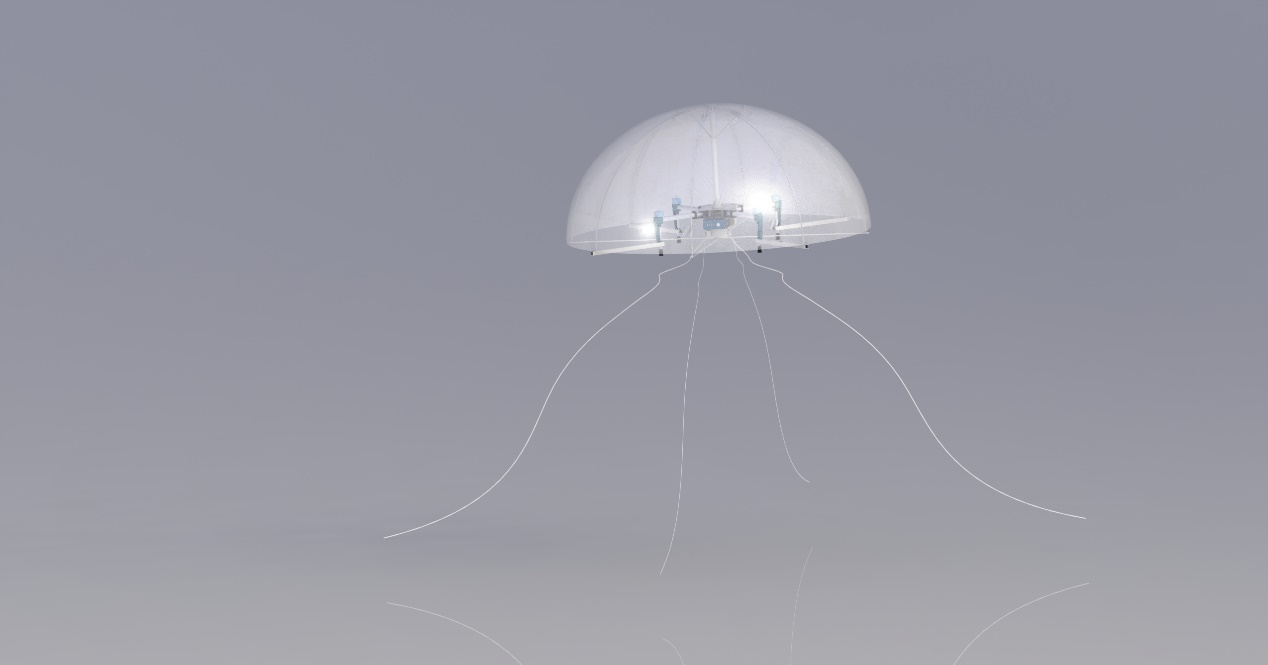
\includegraphics[width = \textwidth]{001}
    \caption{整体渲染图}\par
\end{figure}
本机器人主要由碳纤维骨架搭建而成,大体呈一个600毫米为半径的半球状物体。主要分为机身,支架,触手几个大部分。可以实现在空中的飞行表演和触手的表演动作。机器人由四个螺旋翼提供动力,主要的控制模块,电池,传感器部分都放在机身上。
\begin{figure}[H]
\centering
    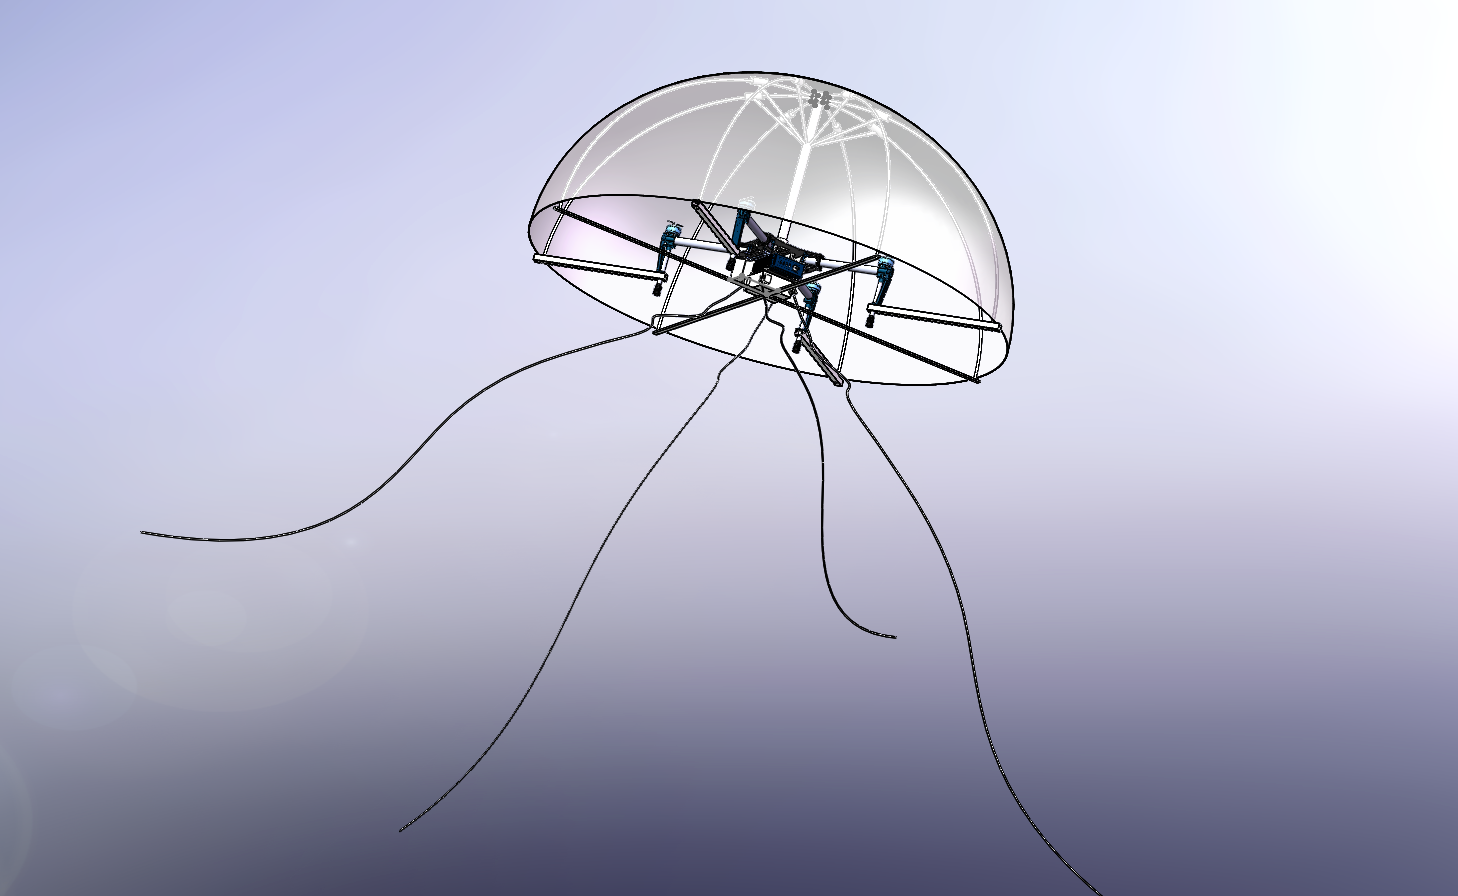
\includegraphics[width = \textwidth]{002}
    \caption{整体渲染图}\par
\end{figure}
\begin{figure}[H]
\centering
    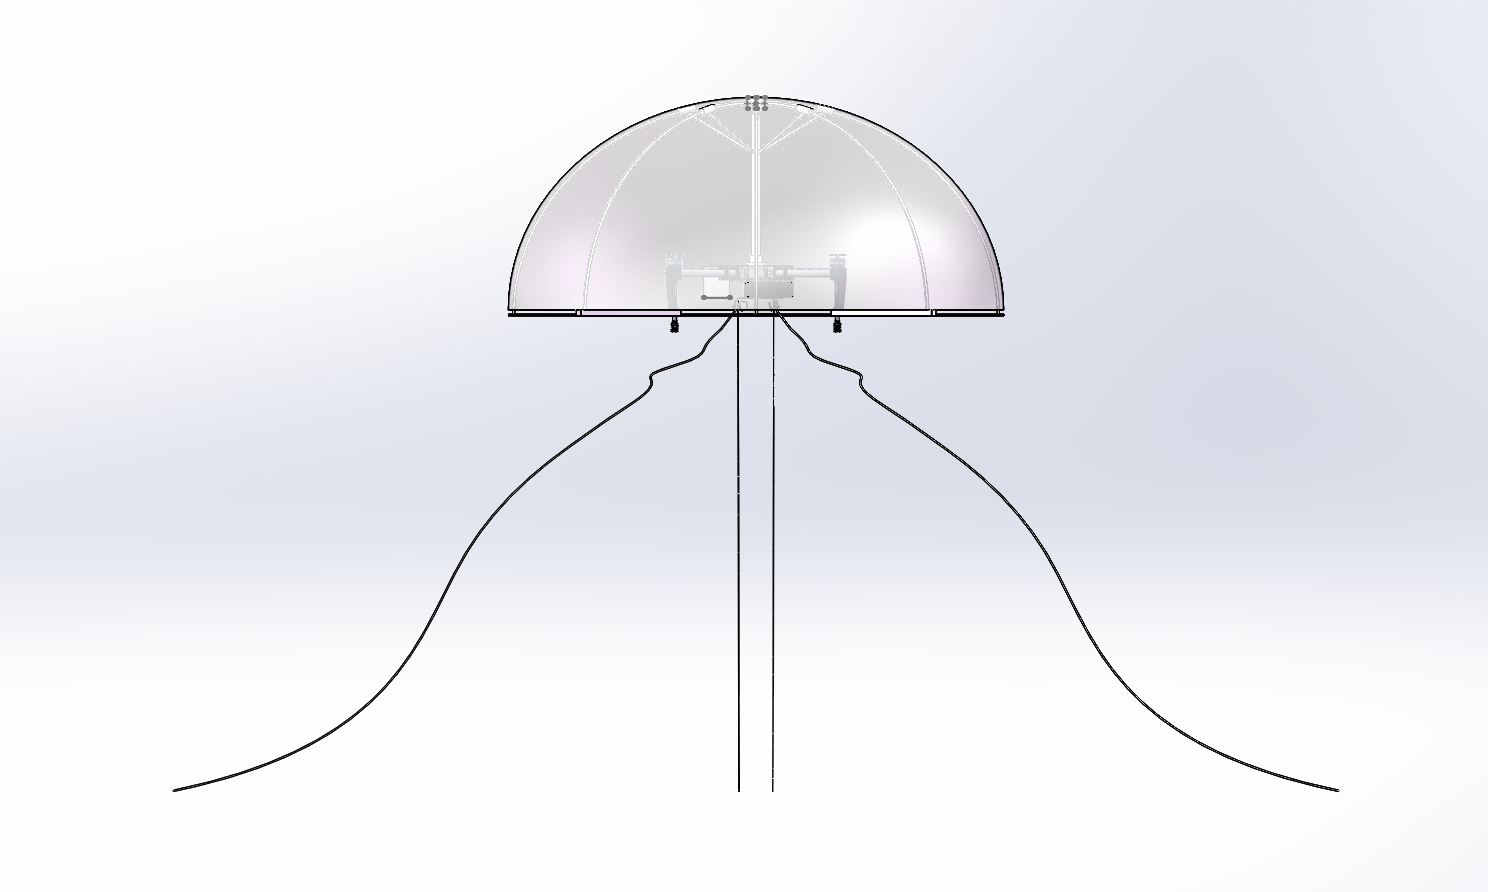
\includegraphics[width = \textwidth]{003}
    \caption{正视图}\par
\end{figure}
\begin{figure}[H]
\centering
    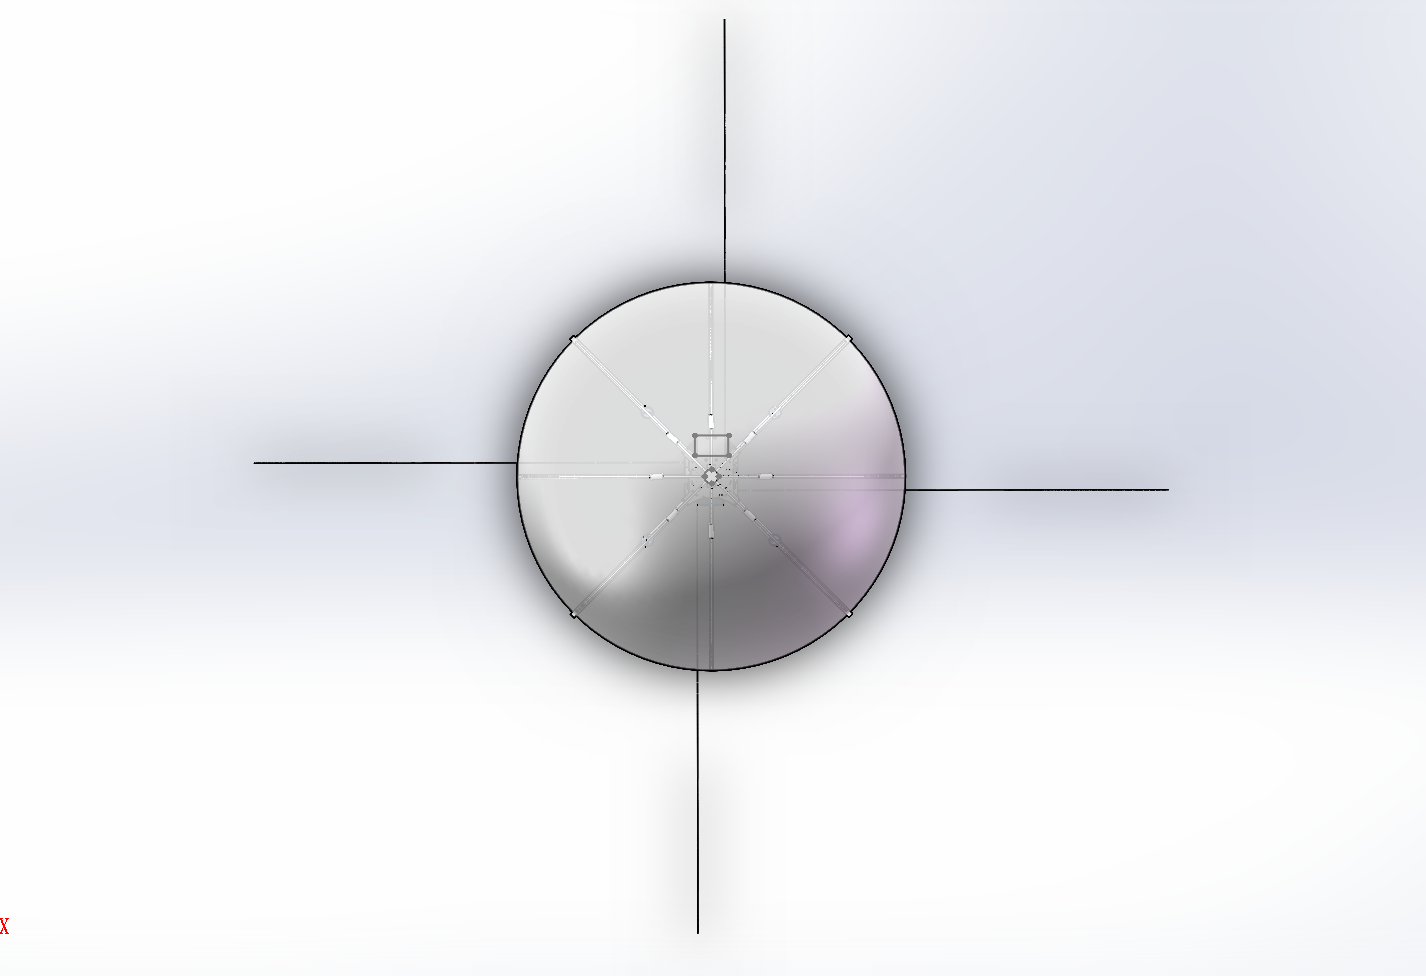
\includegraphics[width = \textwidth]{004}
    \caption{俯视图}\par
\end{figure}
\begin{figure}[H]
\centering
    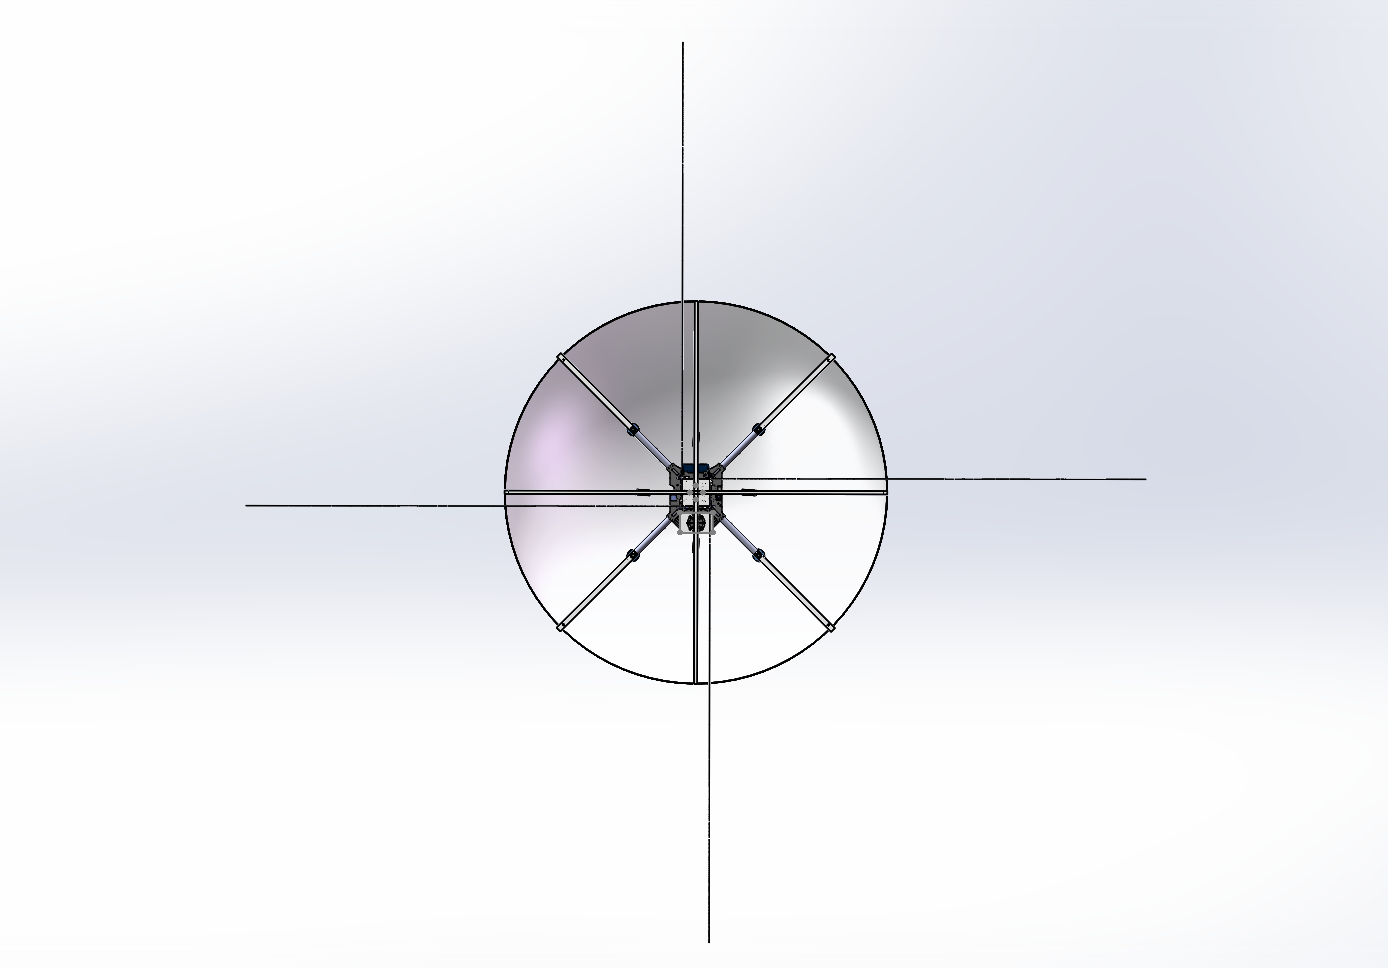
\includegraphics[width = \textwidth]{005}
    \caption{仰视图}\par
\end{figure}
\subsection{飞行原理}
四旋翼飞行器通过调节四个电机转速来改变旋翼转速,实现升力的变化,从而控制飞行器的姿态和位置。四旋翼飞行器是一种六自由度的垂直升降机,但只有四个输入力,同时却有六个状态输出,所以它又是一种欠驱动系统。
\begin{figure}[H]
\centering
    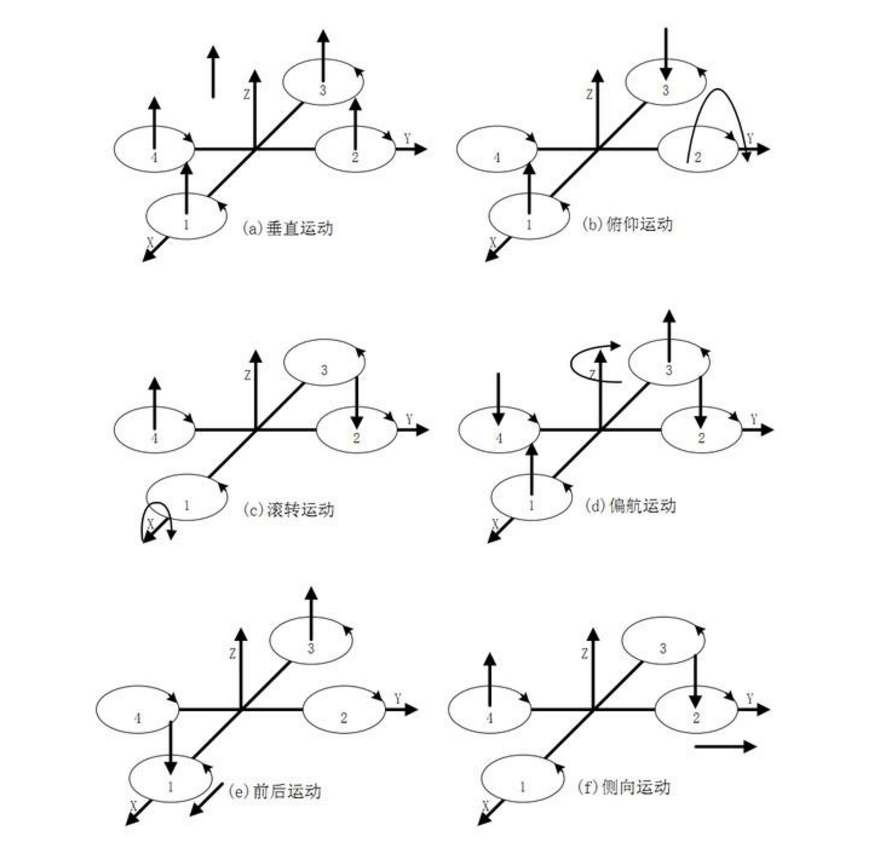
\includegraphics[width = \textwidth]{006}
    \caption{四旋翼飞行器飞行姿态}\par
\end{figure}
四旋翼飞行器的电机 1和电机 3逆时针旋转的同时,电机 2和电机 4顺时针旋转,因此当飞行器平衡飞行时,陀螺效应和空气动力扭矩效应均被抵消。\par
在上图中,电机 1和电机 3作逆时针旋转,电机 2和电机 4作顺时针旋转,规定沿 x轴正方向运动称为向前运动,箭头在旋翼的运动平面上方表示此电机转速提高,在下方表示此电机转速下降。\par
(1)垂直运动:同时增加四个电机的输出功率,旋翼转速增加使得总的拉力增大,当总拉力足以克服整机的重量时,四旋翼飞行器便离地垂直上升;反之,同时减小四个电机的输出功率,四旋翼飞行器则垂直下降,直至平衡落地,实现了沿 z轴的垂直运动。当外界扰动量为零时,在旋翼产生的升力等于飞行器的自重时,飞行器便保持悬停状态。\par 
(2)俯仰运动:在图(b)中,电机 1的转速上升,电机 3 的转速下降(改变量大小应相等),电机 2、电机 4 的转速保持不变。由于旋翼1 的升力上升,旋翼 3 的升力下降,产生的不平衡力矩使机身绕 y 轴旋转,同理,当电机 1 的转速下降,电机 3的转速上升,机身便绕y轴向另一个方向旋转,实现飞行器的俯仰运动。\par
(3)滚转运动:与图 b 的原理相同,在图 c 中,改变电机 2和电机 4的转速,保持电机1和电机 3的转速不变,则可使机身绕 x 轴旋转(正向和反向),实现飞行器的滚转运动。\par
(4)偏航运动:旋翼转动过程中由于空气阻力作用会形成与转动方向相反的反扭矩,为了克服反扭矩影响,可使四个旋翼中的两个正转,两个反转,且对角线上的各个旋翼转动方向相同。反扭矩的大小与旋翼转速有关,当四个电机转速相同时,四个旋翼产生的反扭矩相互平衡,四旋翼飞行器不发生转动;当四个电机转速不完全相同时,不平衡的反扭矩会引起四旋翼飞行器转动。在图 d中,当电机 1和电机 3 的转速上升,电机 2 和电机 4 的转速下降时,旋翼 1和旋翼3对机身的反扭矩大于旋翼2和旋翼4对机身的反扭矩,机身便在富余反扭矩的作用下绕 z轴转动,实现飞行器的偏航运动,转向与电机 1、电机3的转向相反。\par
(5)前后运动:要想实现飞行器在水平面内前后、左右的运动,必须在水平面内对飞行器施加一定的力。在图 e中,增加电机 3转速,使拉力增大,相应减小电机 1转速,使拉力减小,同时保持其它两个电机转速不变,反扭矩仍然要保持平衡。按图 b的理论,飞行器首先发生一定程度的倾斜,从而使旋翼拉力产生水平分量,因此可以实现飞行器的前飞运动。向后飞行与向前飞行正好相反。(在图 b 图 c中,飞行器在产生俯仰、翻滚运动的同时也会产生沿 x、y轴的水平运动。\par
(6)倾向运动:在图 f 中,由于结构对称,所以倾向飞行的工作原理与前后运动完全一样。\par
\subsection{各模块详解}
\subsubsection{薄膜骨架}
\begin{figure}[H]
\centering
    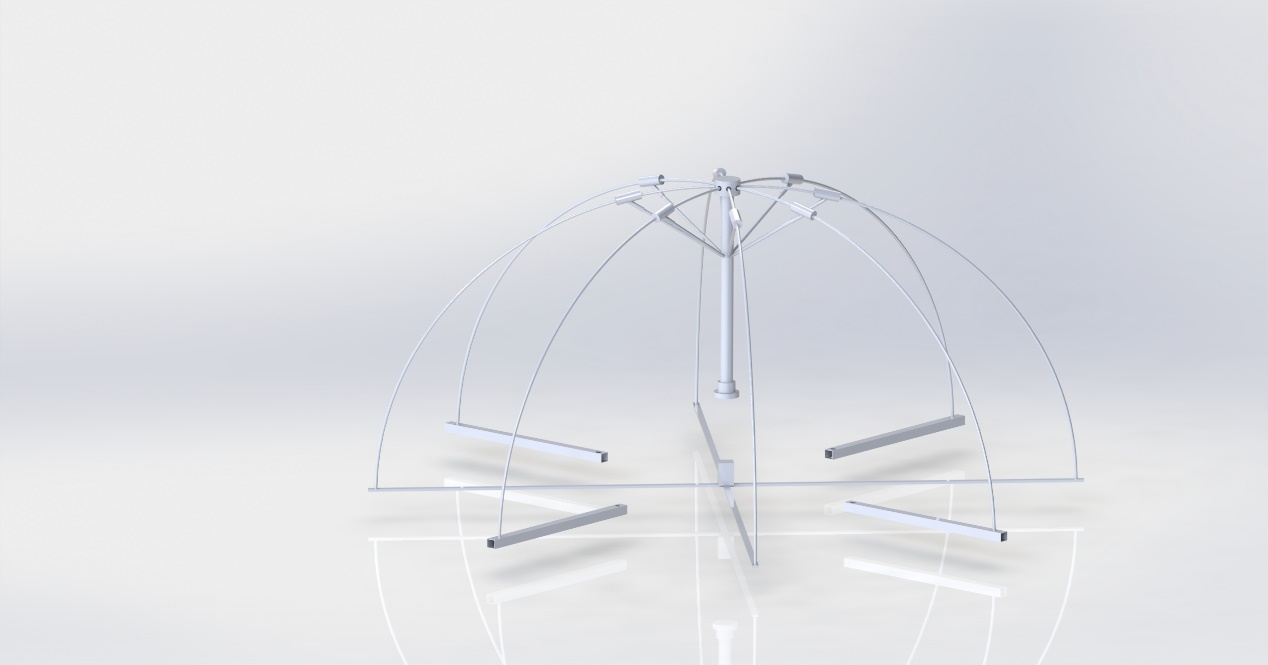
\includegraphics[width = \textwidth]{007}
    \caption{薄膜骨架}\par
\end{figure}
此装置的功能是用来支撑薄膜,在实际情况下会以该个骨架为支撑覆盖一层薄膜。骨架由位于轴线的支柱和下面伸出的四个管来支持重量。下面向内伸出的四根管子将会绑定在机身的四个落地杆上。
\begin{figure}[H]
\centering
    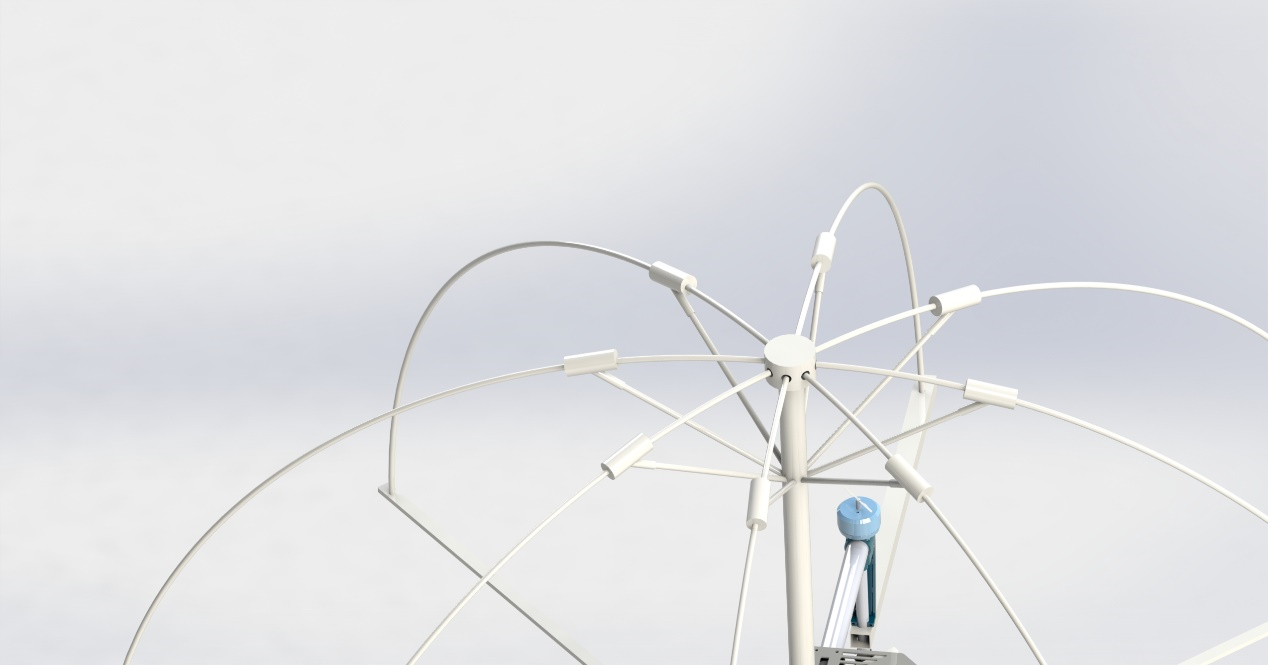
\includegraphics[width = \textwidth]{008}
    \caption{骨架细节图}\par
\end{figure}
从中间的支柱上伸出8个细杆用来固定支撑杆,这样整个支撑架将会更加牢固。
\subsubsection{旋翼}
\begin{figure}[H]
\centering
    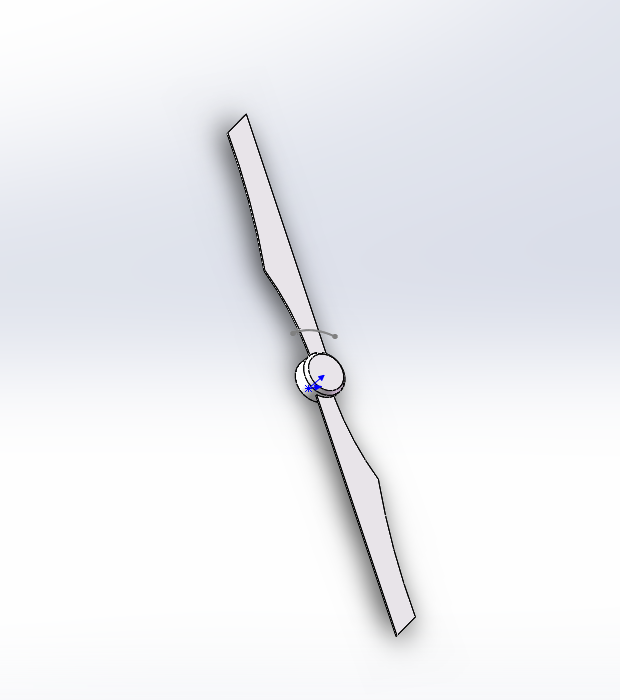
\includegraphics[width = \textwidth]{009}
    \caption{旋翼}\par
\end{figure}
扇叶的形状如图所示,半径约340mm,扇叶侧面呈流线型,扇叶内称大角度的螺旋状,螺距为25cm,飞行器飞行时靠4个扇叶转动提供升力,依靠部分扇叶转速降低来控制方向。扇叶转动依靠在其下面的电机提供动力。\par
机翼采用正反桨,原理如下。\par
\begin{figure}[H]
\centering
    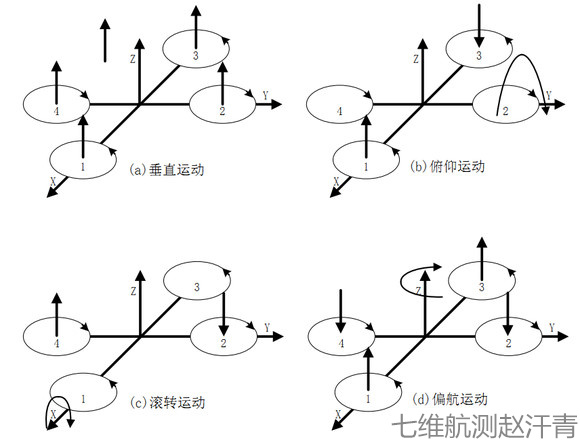
\includegraphics[width = \textwidth]{010}
    \caption{正反桨原理}\par
\end{figure}
每个螺旋桨在旋转的时候跟空气摩擦,会产生水平的扭矩。所以需要让几个螺旋桨沿相反方向旋转,让力矩互相抵消。\par
\subsubsection{机身部分}
\begin{figure}[H]
\centering
    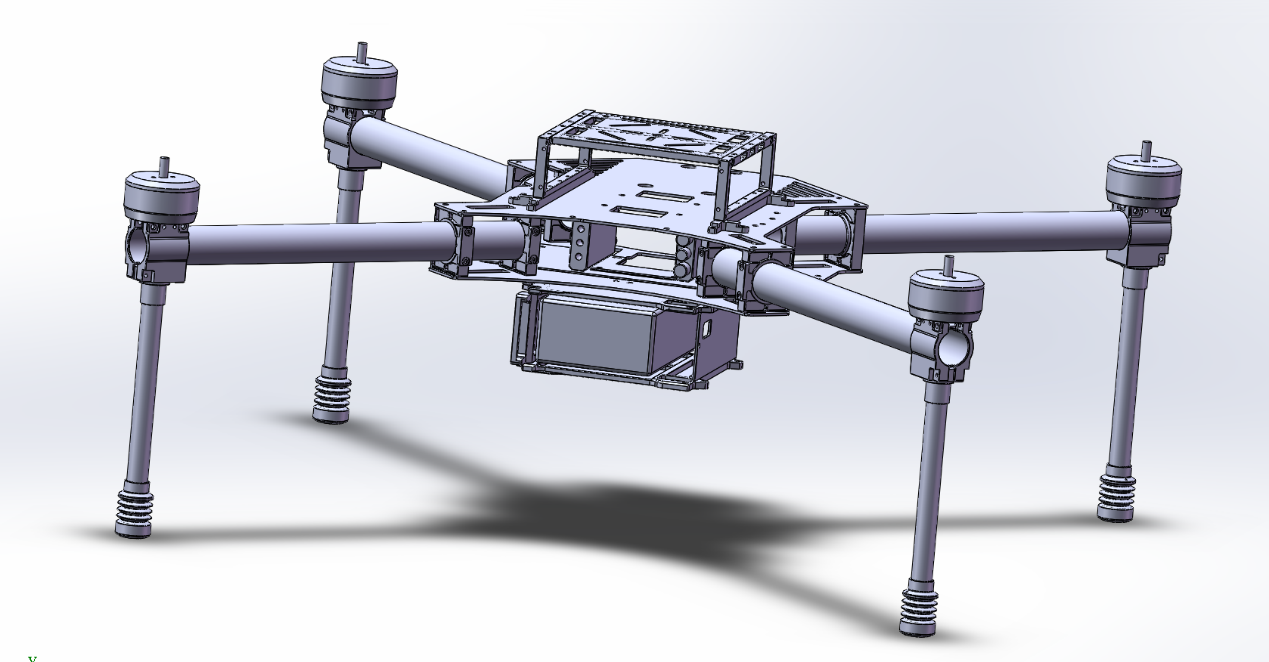
\includegraphics[width = \textwidth]{011}
    \caption{机身整体图}\par
\end{figure}
这是除去支撑骨架和旋翼的机身部分,下面将对其进行拆分。
\subsubsection{四脚}
\begin{figure}[H]
\centering
    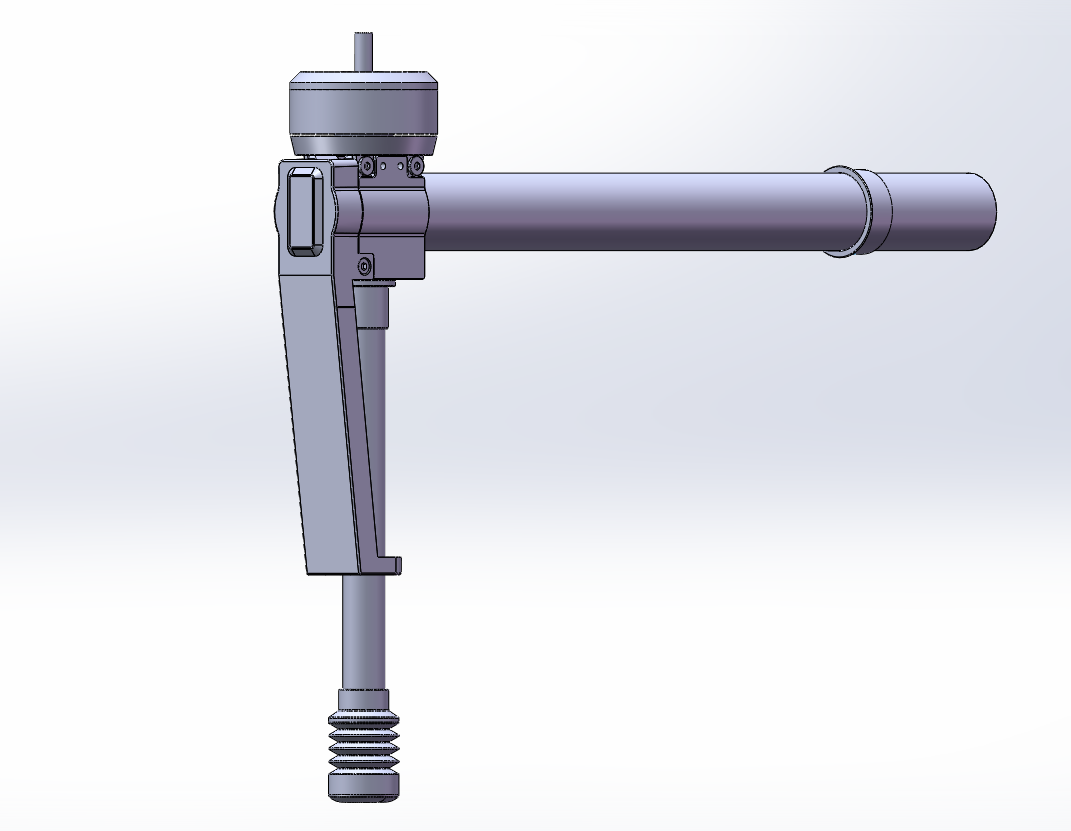
\includegraphics[width = \textwidth]{012}
    \caption{四脚细节图}\par
\end{figure}
如图所示,四个脚由多个部分组成,分别为连接杆,落地杆,电机和固定部分几个部分。连接杆用来连接后面的几个部分。固定部分用来将电机和落地杆固定在连接杆上。电机固定在了连接杆之上,用来驱动电机。落地杆下方有一个弹性结构,可以有效减少落地时候收到的冲力。
\subsubsection{机身}
\begin{figure}[H]
\centering
    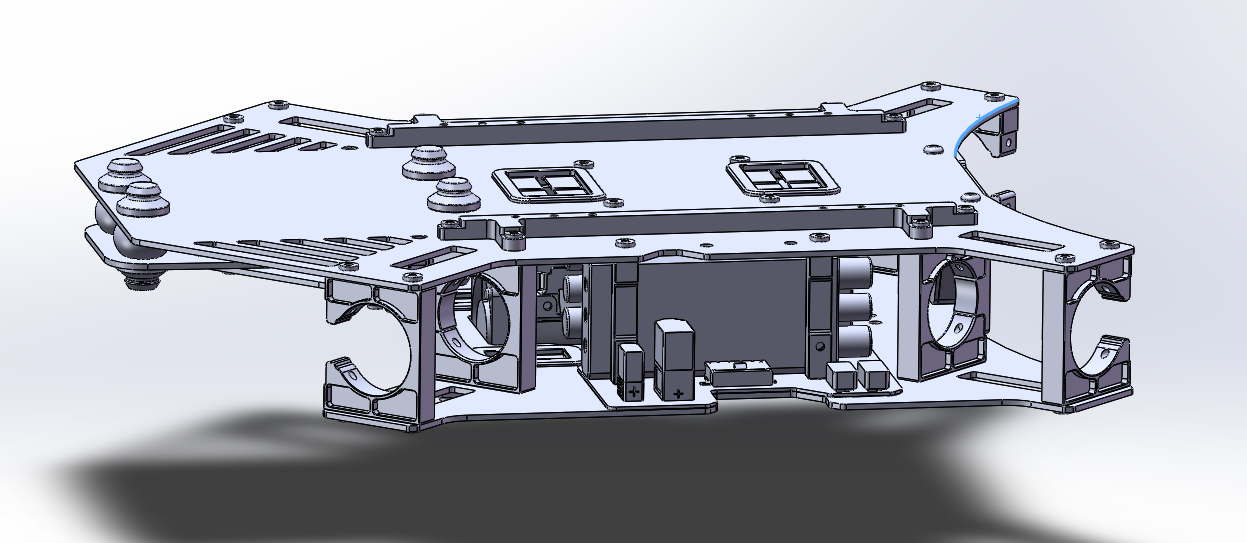
\includegraphics[width = \textwidth]{013}
    \caption{机身细节图}\par
\end{figure}
\begin{figure}[H]
\centering
    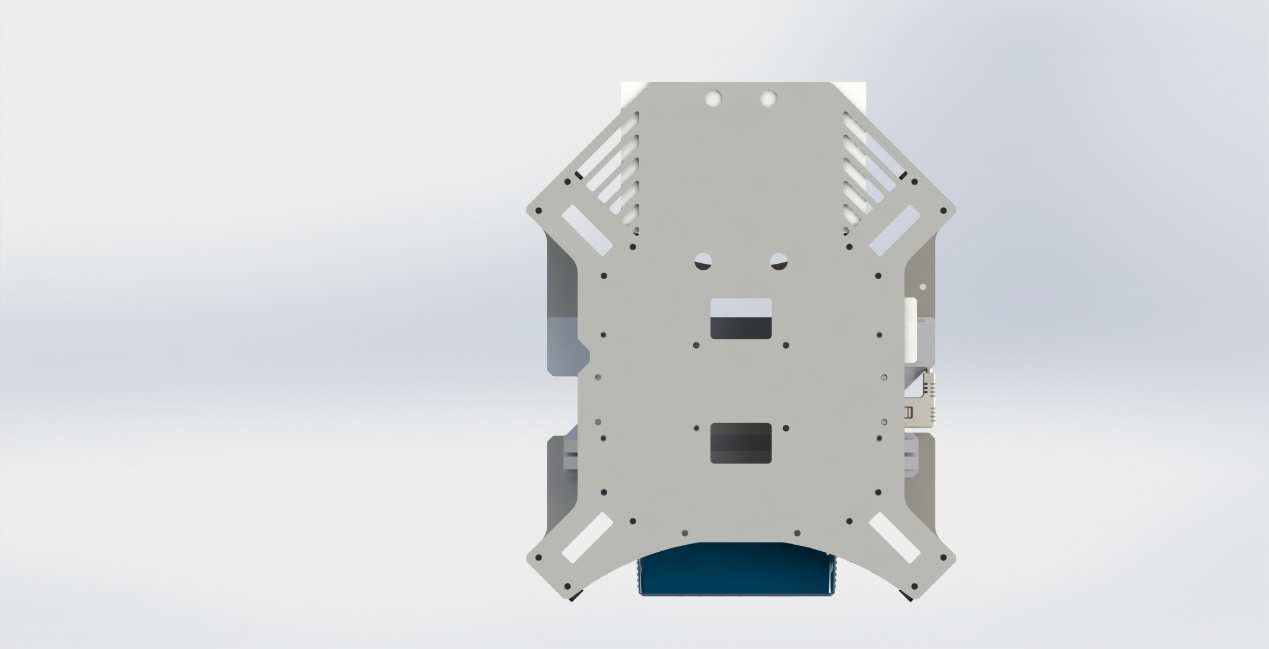
\includegraphics[width = \textwidth]{014}
    \caption{机身细节图}\par
\end{figure}
\begin{figure}[H]
\centering
    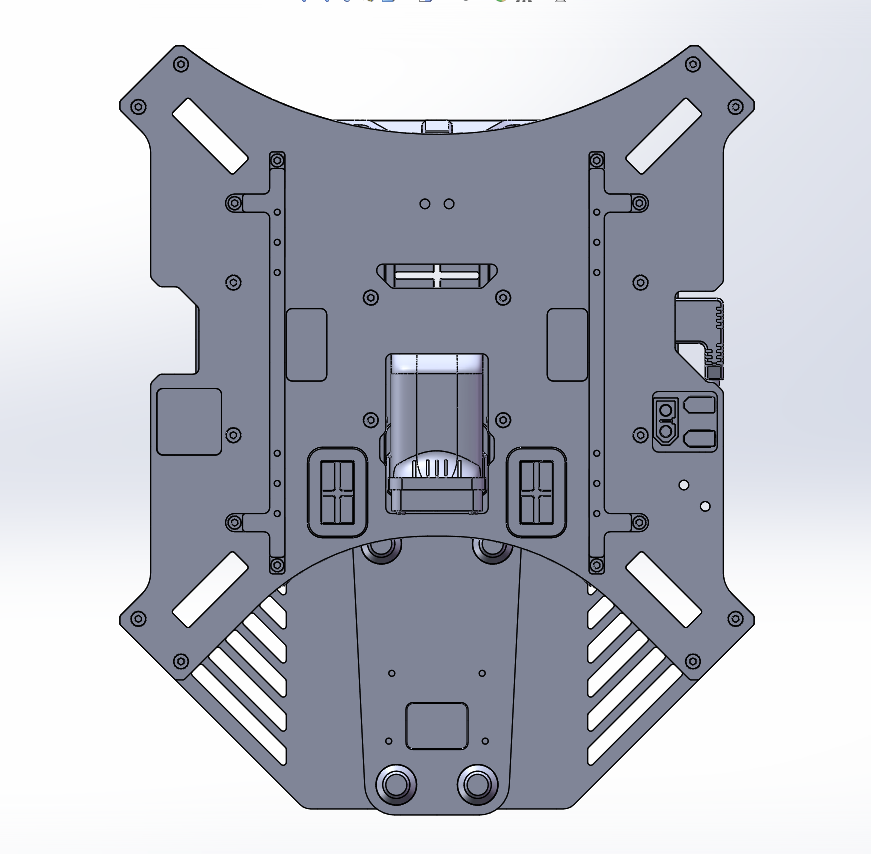
\includegraphics[width = \textwidth]{015}
    \caption{机身细节图}\par
\end{figure}
机身是全机器最重要的部分,其主要功能是容纳各个元件,包括主控板,电调,电池以及各种传感器元件。机身大小约293mm*210.38mm\par
机身内部有四个凹槽用来固定电调,在下面板处放置飞行控制板和各种传感器。机身带有预留的几个风扇模块分别进行散热等工作。\par
具体的内容部分将在电路部分解释。
\subsubsection{触手}
\begin{figure}[H]
\centering
    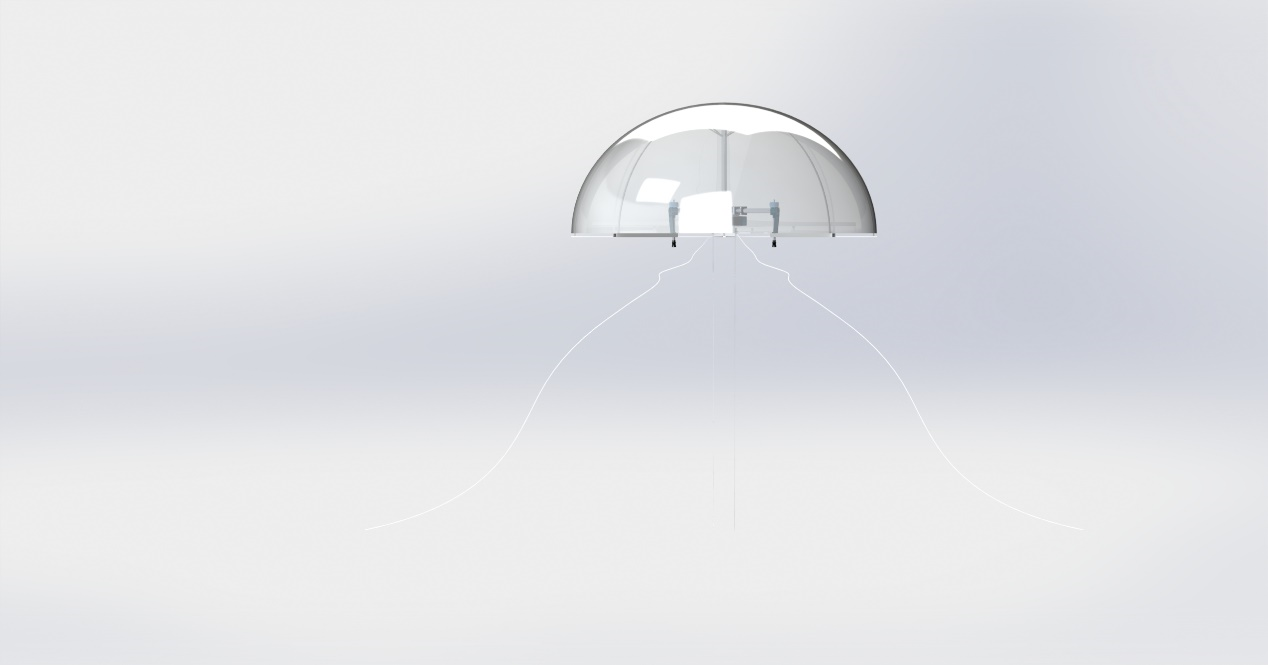
\includegraphics[width = \textwidth]{016}
    \caption{触手效果图}\par
\end{figure}
触手部分主要用于表演,四个触手是可以在一定程度上控制的,这样就可以通过预先给定的程序产生所需要的表演效果。
\begin{figure}[H]
\centering
    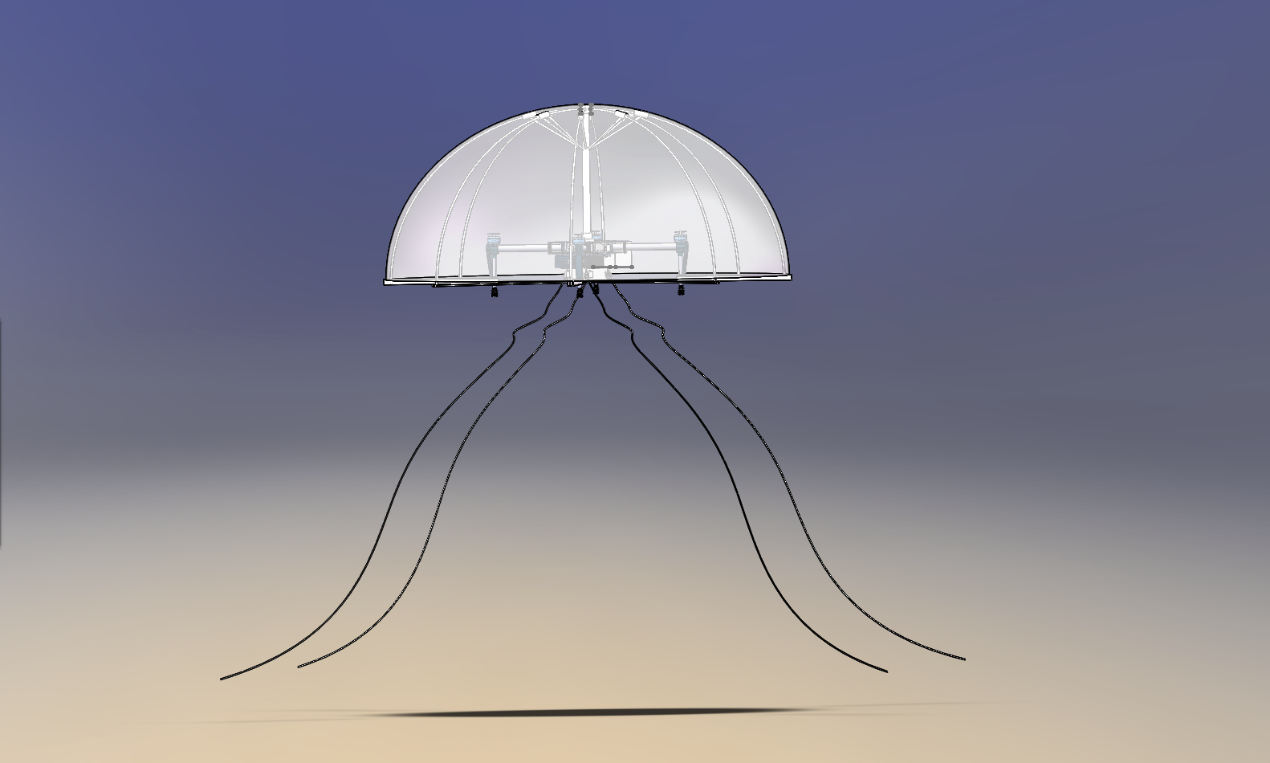
\includegraphics[width = \textwidth]{017}
    \caption{触手效果图}\par
\end{figure}
\begin{figure}[H]
\centering
    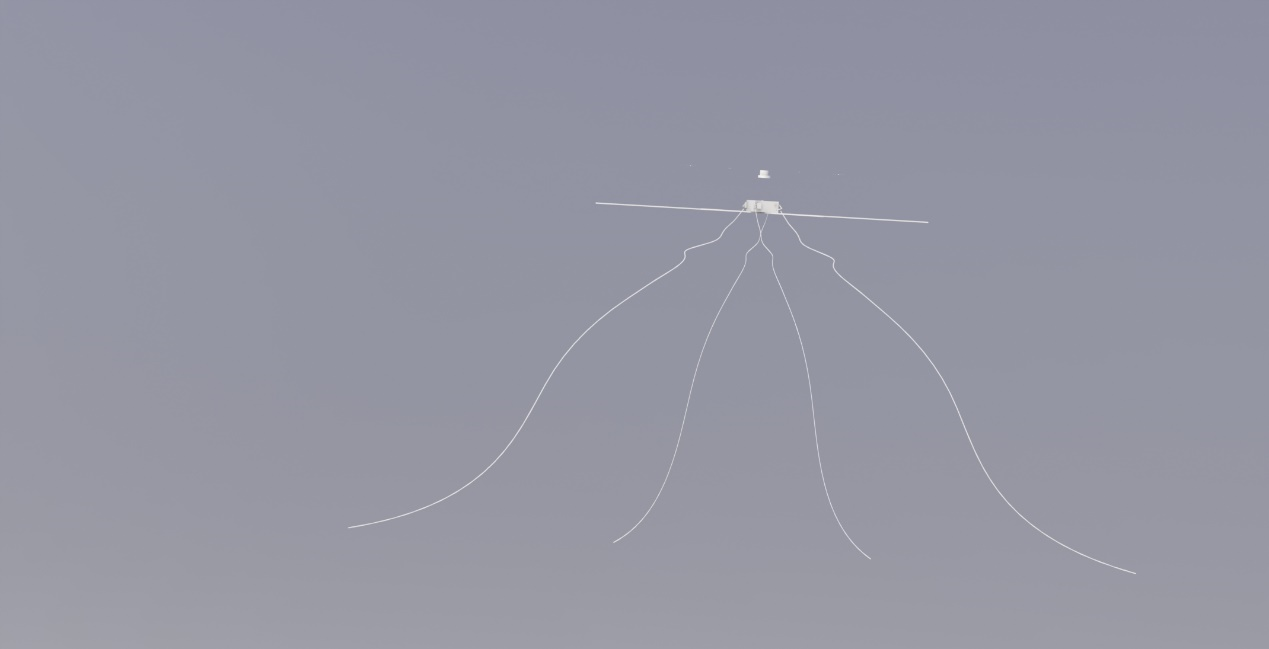
\includegraphics[width = \textwidth]{018}
    \caption{触手细节图}\par
\end{figure}
在机身电池的下方有一个舵机控制模块,由四个舵机及相应的控制电路组成。每个舵机都连接了一个曲柄摇杆结构,触手由曲柄摇杆结构控制,在舵机的控制下进行飘动。
\begin{figure}[H]
\centering
    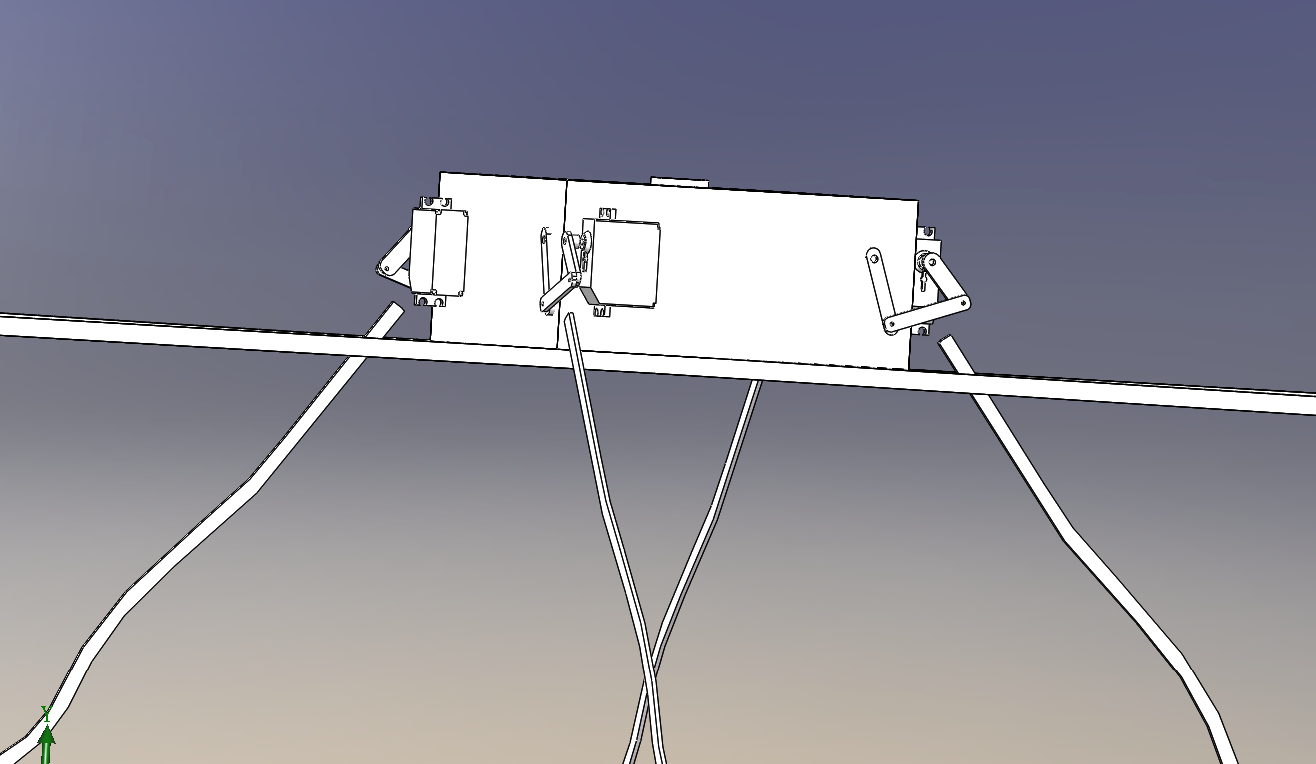
\includegraphics[width = \textwidth]{019}
    \caption{触手控制模块}\par
\end{figure}
上图是具体的控制部分,其原理可以由下面的原理图解释。
\begin{figure}[H]
\centering
    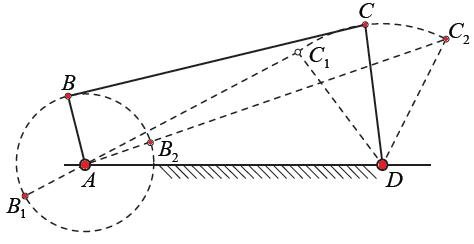
\includegraphics[width = \textwidth]{020}
    \caption{触手控制原理图}\par
\end{figure}
原理解释: 两个连架杆中,一为曲柄,一为摇杆。通常曲柄主动,摇杆从动,但也有摇杆主动的情况。\par  
当曲柄匀速转动时,摇杆作变速摆动,而且往复摆动的平均速度是不同的。若将平均速度小的行程作为工作行程(正行程),将平均速度大的行程作为非工作行程(反行程),那么,我们把曲柄摇杆机构这种正、反行程平均速度不等的特性称为急回特性。急回特性很有用,牛头刨床、往复式运输机等机械就常常利用急回特性来缩短非生产时间,提高生产率。
\section{电路结构设计}
\subsection{电池部分}
考虑到载重实体重量较大,鉴于需要为飞行部分提供较大升力,故需要选用较大容量与功率的电池,我们选用锂聚合物电池。
选用:格氏ACE 4000mAh 14.8V 4S 25C 锂聚合物电池\par
以下为原物图:\par
\begin{figure}[H]
\centering
    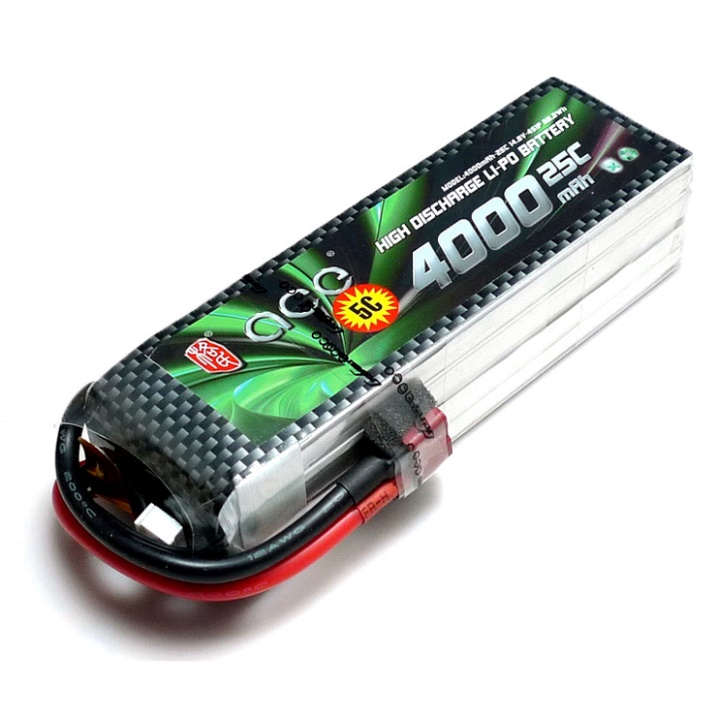
\includegraphics[width = \textwidth]{021}
    \caption{电池}\par
\end{figure}
相关参数:\par
\begin{center}
\begin{longtable}{|c|c|c|}
\hline
\multicolumn{3}{|c|}{技术参数}\\
\hline
包装&\multicolumn{2}{c|}{防震气泡袋、硬纸盒}\\
\hline
电芯&\multicolumn{2}{c|}{锂聚合物动力电芯}\\
\hline
容量&\multicolumn{2}{c|}{4000mah}\\
\hline
电压&\multicolumn{2}{c|}{22.2V}\\
\hline
持续放电倍率&\multicolumn{2}{c|}{250C}\\
\hline
\multirow{2}{*}{大约体积}&长&13.7厘米\\
\cline{2-3}
&宽&4.1厘米\\
\hline
&厚&3.3厘米\\
\hline
大约重量&\multicolumn{2}{c|}{425克}\\
\hline
\multirow{2}{*}{大约线长}&主电力线&10厘米\\
\cline{2-3}
&平衡线&5厘米\\
\hline
\end{longtable}
\end{center}
\subsection{传感器部分}
\subsubsection{红外光电传感器}
原理:光电传感器是通过把光强度的变化转换成电信号的变化来实现控制的。光电传感器在一般情况下,有三部分构成,它们分为:发送器、接收器和检测电路。\par
发送器对准目标发射光束,发射的光束一般来源于半导体光源,发光二极管(LED)、激光二极管及红外发射二极管。光束不间断地发射,或者改变脉冲宽度。接收器有光电二极管、光电三极管、光电池组成。在接收器的前面,装有光学元件如透镜和光圈等。在其后面是检测电路,它能滤出有效信号和应用该信号。\par
\begin{figure}[H]
\centering
    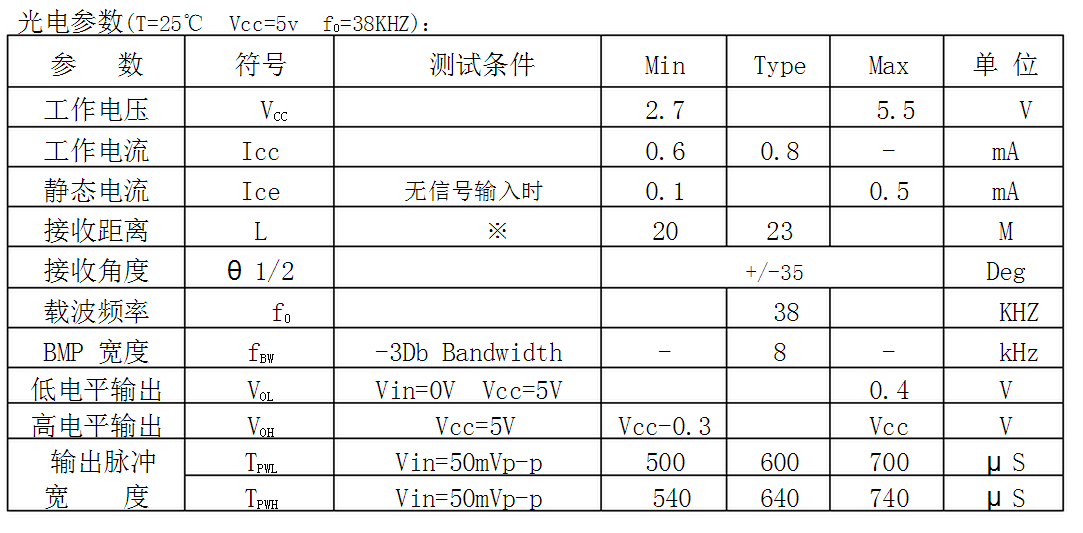
\includegraphics[width = \textwidth]{022}
    \caption{光电参数}\par
\end{figure}
\begin{figure}[H]
\centering
    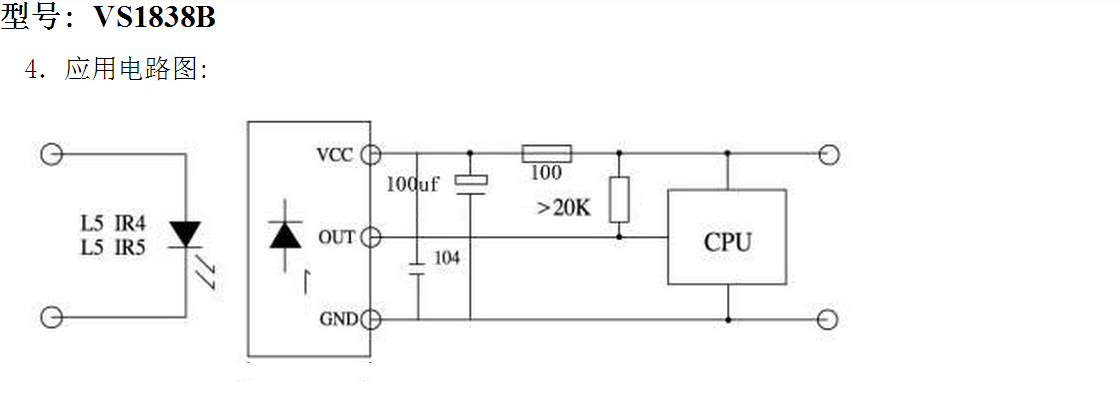
\includegraphics[width = \textwidth]{023}
    \caption{电路图}\par
\end{figure}
\begin{figure}[H]
\centering
    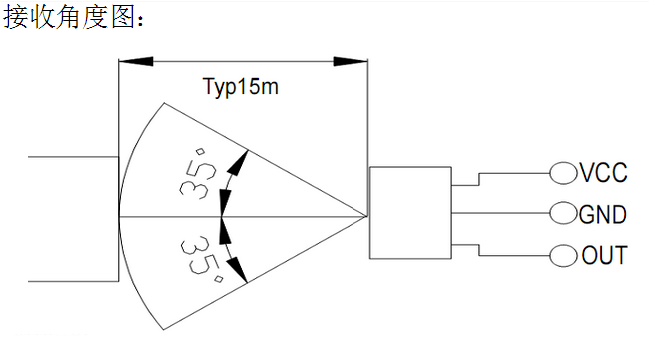
\includegraphics[width = \textwidth]{024}
    \caption{电路图}\par
\end{figure}
\begin{figure}[H]
\centering
    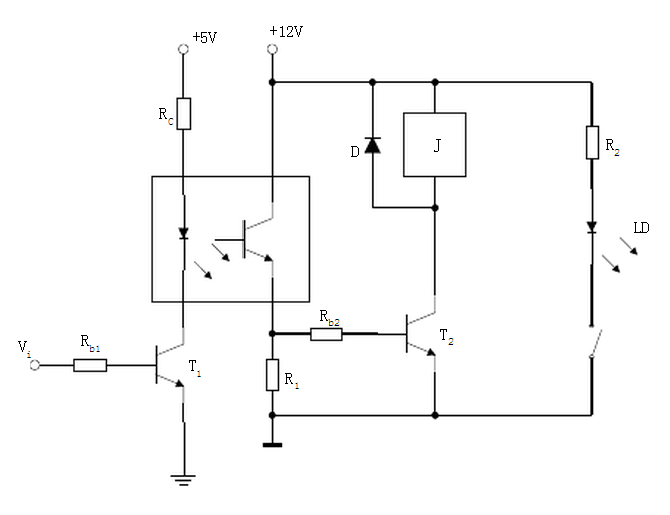
\includegraphics[width = \textwidth]{025}
    \caption{电路图}\par
\end{figure}
选择使用红外光电开关——漫反射式避障传感器,暂定Gaston E18-D80NK。\par
以下为实物图:\par
\begin{figure}[H]
\centering
    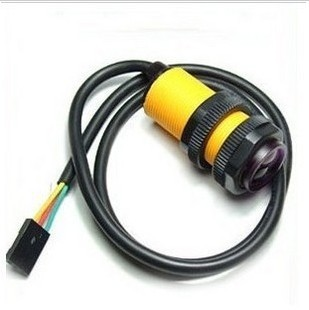
\includegraphics[width = \textwidth]{026}
    \caption{实物图:E18-D80NK}\par
\end{figure}
这是一种集发射与接收于一体的光电传感器。检测距离可以根据要求进行调节。该传感器具有探测距离远、受可见光干扰小、价格便宜、易于装配、使用方便等特点,可以广泛应用于机器人避障、流水线计件等众多场合。
\begin{center}
\begin{longtable}{|c|c|}
\hline
电器特性&U:5VDC\\
&I:100mA\\
&Sn:3-80CM\\
\hline
尺寸&直径:17MM\\
&传感器长度:70MM\\
&引线长度:120MM\\
\hline
引脚&红色正极\\
&黑色信号\\
&兰色负极\\
\hline
\end{longtable}
\end{center}
光电开关E18的技术参数:\par
\begin{center}
\begin{longtable}{|c|c|}
\hline
输出电流 DC/SCR&100mA/5V\\
\hline
消耗电流&DC<25mA\\
\hline
响应时间&<2ms\\
\hline
指向角&<=$15^{\circ}$ ,有效距离3-80CM可调\\
\hline
检测物体&透明或不透明体\\
\hline
工作环境温度&$-25^{\circ}C~+55^{\circ}C$\\
\hline
标准检测物体&太阳光10000LX以下,白炽灯3000LX以下\\
\hline
外壳材料&塑料\\
\hline
\end{longtable}
\end{center}
\subsubsection{超声波传感器}
原理:超声波传感器是利用超声波的特性研制而成的传感器。超声波是一种振动频率高于声波的机械波,由换能晶片在电压的激励下发生振动产生的,它具有频率高、波长短、绕射现象小,特别是方向性好、能够成为射线而定向传播等特点。\par
\begin{figure}[H]
\centering
    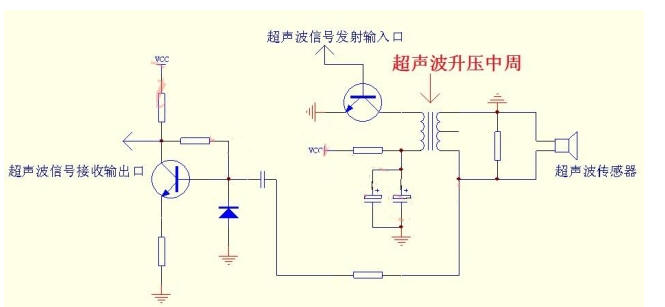
\includegraphics[width = \textwidth]{027}
    \caption{efr40rs型号超声波传感器}\par
\end{figure}
\begin{figure}[H]
\centering
    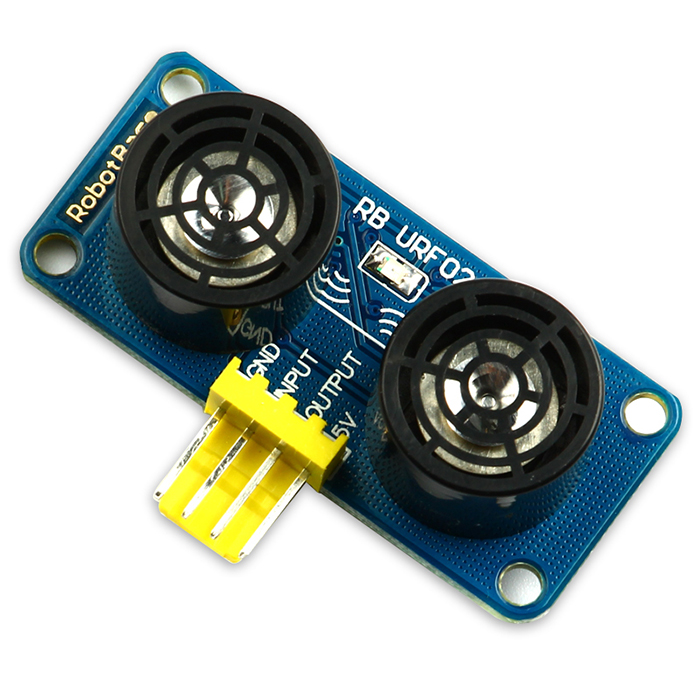
\includegraphics[width = \textwidth]{028}
    \caption{RB URF02超声波传感器}\par
\end{figure}
\begin{figure}[H]
\centering
    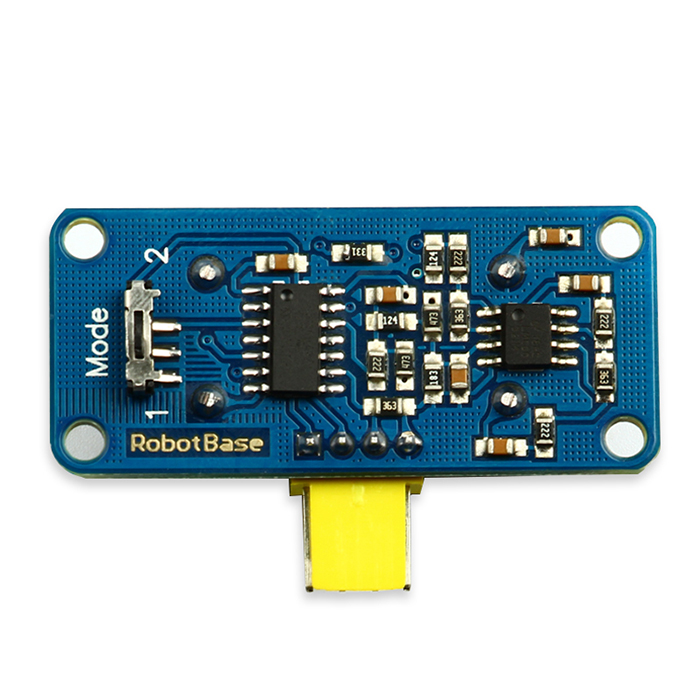
\includegraphics[width = \textwidth]{029}
    \caption{RB URF02超声波传感器}\par
\end{figure}
\begin{center}
\begin{longtable}{|c|c|}
\hline
工作电压&+5V\\
\hline
工作电流&<20mA\\
\hline
工作频率&40KHz\\
\hline
探测有效距离&1cm~500cm\\
\hline
探测分辨率&0.5cm\\
\hline
工作环境温度&$-10^{\circ}C~+70^{\circ}C$\\
\hline
探测误差&$\pm$0.5\%\\
\hline
灵敏度&大于1.8m外可以探测到直径2cm物体\\
\hline
接口类型&TTL\\
\hline
方向性侦测范围&定向式(水平/垂直)65度圆锥\\
\hline
尺寸大小&46.7mm*25.7mm*19mm\\
\hline
重量大小&5g\\
\hline
\end{longtable}
\end{center}
\subsubsection{无线摄像头}
为了尽量降低机载重量,再三比较之下,我们选用萤石((EZVIZ)C3C高清夜视 智能无线网络摄像头)
\begin{figure}[H]
\centering
    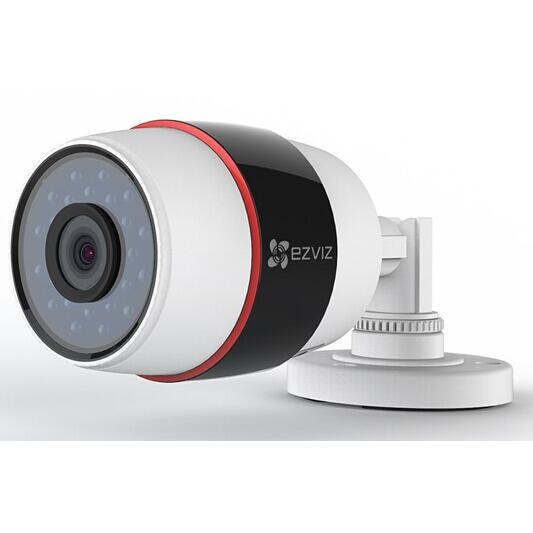
\includegraphics[width = \textwidth]{030}
    \caption{摄像头实物图}\par
\end{figure}
相关参数:
\begin{center}
\begin{longtable}{|c|c|}
\hline
型号	&CS-C3C-31WFR(4mm)\\
\hline
颜色	&白色\\
\hline
类型	&CMOS壁挂式互联网摄像机\\
\hline
系统支持	&iphone、android、windows、web\\
\hline
操作方式	&手机APP/PC/WEB端都可控制\\
\hline
使用环境温度	&-30℃~60℃,湿度小于95\%(无凝结)\\
\hline
存储类型	&支持Micro SD卡(最大128G)\\
\hline
功率W	&5W MAX(ICR切换瞬间7W)\\
\hline
工作环境	&红外照射距离30米\\
\hline
机身尺寸	&173mm*83.5mm*69.8mm\\
\hline
机身重量	&322克\\
\hline
特点	&IP66防水防尘等级,支持WIFI,萤石自适应存储技术\\
\hline

\end{longtable}
\end{center}

\subsubsection{飞控板}
飞控见程序部分
\subsubsection{电机电路}
本实验控制四个扇叶需要用到电机电路。\par
风扇电机调速电路图:
\begin{figure}[H]
\centering
    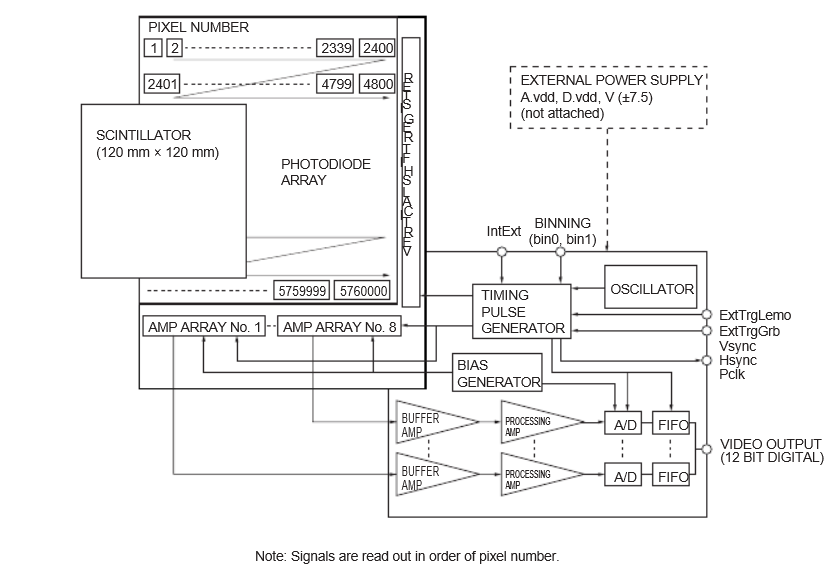
\includegraphics[width = \textwidth]{031}
    \caption{C7942CK-12电调电路}\par
\end{figure}
\begin{figure}[H]
\centering
    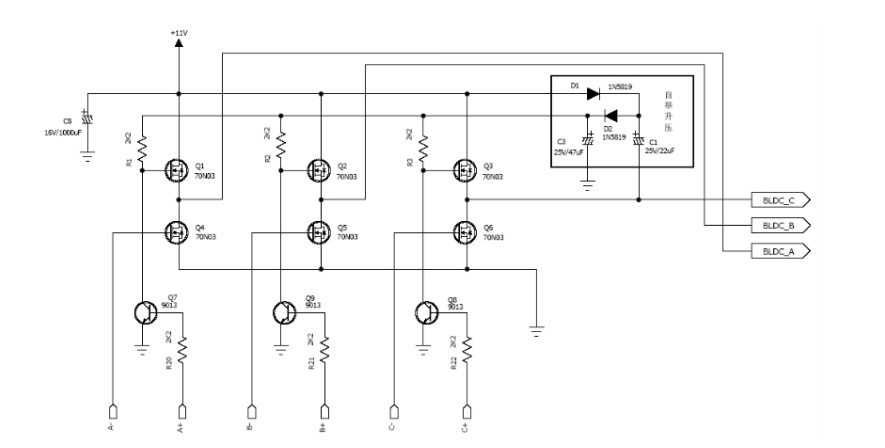
\includegraphics[width = \textwidth]{032}
    \caption{无刷电机三相驱动桥}\par
\end{figure}
上图为三相全桥驱动电路,使用6个N沟道的MOSFET管(Q1~Q6)作功率输出文件,工作时输出电流达数十安。图中R1,R2,R3为Q1、Q2、Q3的上位电阻,为上臂驱动管提供两倍于电源电压的上拉电平,使上臂MOSFET管在工作时有足够的Vgs差,降低MOSFET管导通时的内阻。
\begin{figure}[H]
\centering
    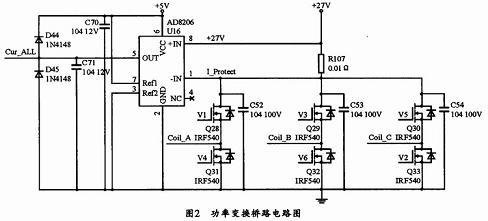
\includegraphics[width = \textwidth]{033}
    \caption{功率变换桥路电路图}\par
\end{figure}
\section{程序部分}
机器人总体控制关系如图:
\begin{figure}[H]
\centering
    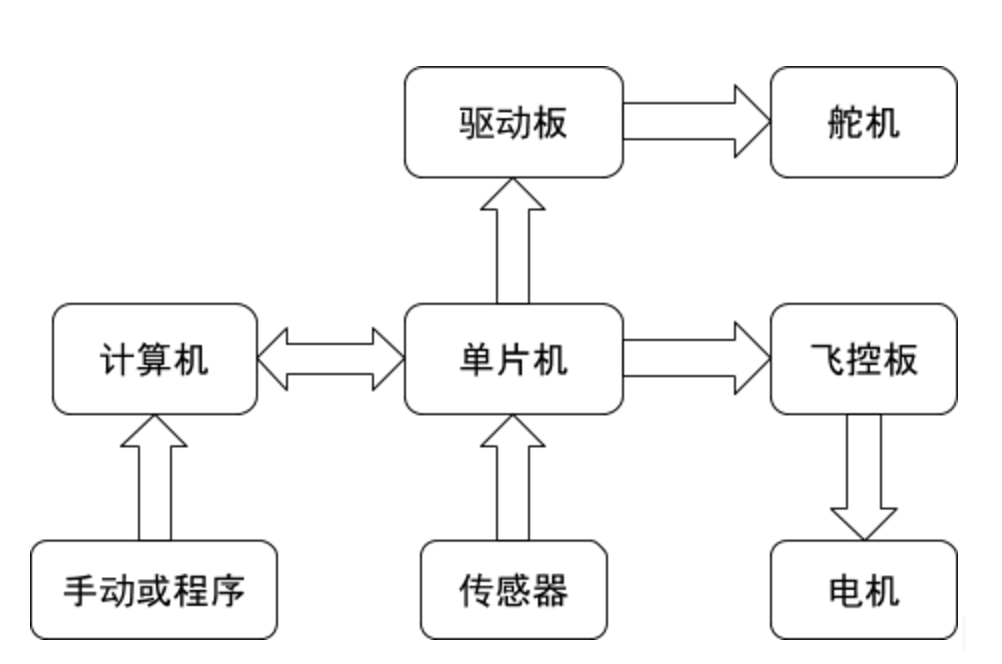
\includegraphics[width = \textwidth]{034}
    \caption{总体控制关系图}\par
\end{figure}
机器人以单片机为中心,传感器的数据通过单片机传递给计算机,由计算机完成计算,将需要完成的动作传递给单片机,由单片机发出控制信号,控制电机和舵机完成动作。\par
	由于过于复杂的硬件会影响可靠性,并且会使机器的耗电量大大增加。所以我们决定,用简单的硬件完成频率最高、最基本的工作,而更复杂的功能由软件实现。
\subsection{单片机}
单片机是各个部件间通信、控制的枢纽,所以也是最重要的部分。综合各种因素考虑,我们打算采用树莓派3B。
\begin{figure}[H]
\centering
    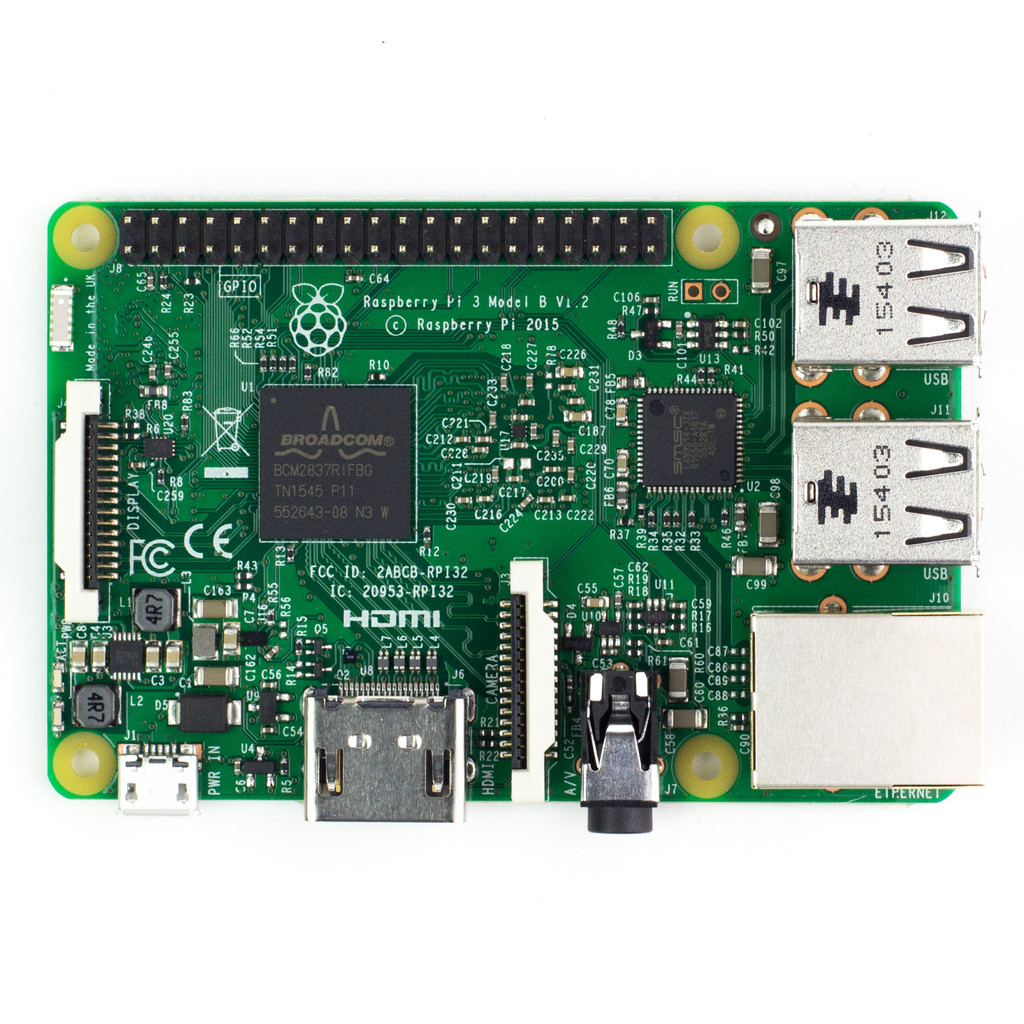
\includegraphics[width = \textwidth]{035}
    \caption{树莓派3B}\par
\end{figure}
主要参数:
\begin{center}
\begin{itemize}
\item Broadcom BCM2837 芯片组,运行频率 1.2 GHz
\item 64 位四核 ARM Cortex-A53
\item 802.11 b/g/n 无线局域网
\item 蓝牙 4.1
\item 双核 Videocore IV® 多媒体协处理器
\item 1 GB LPDDR2 存储器
\item 支持所有最新的 ARM GNU/Linux 分发和 Windows 10 IoT
\item MicroUSB 连接器,用于 2.5 A 电源
\item 1 x 10/100 以太网端口
\item 1 x HDMI 视频/音频连接器
\item 1 x RCA 视频/音频连接器
\item 1 x CSI 摄像机连接器
\item 4 个 USB 2.0 端口
\item 40 个 GPIO 引脚
\item 芯片天线
\item DSI 显示连接器
\item microSD 卡插槽
\item 尺寸:85 x 56 x 17 mm
\end{itemize}
\end{center}
电路图:
\begin{figure}[H]
\centering
    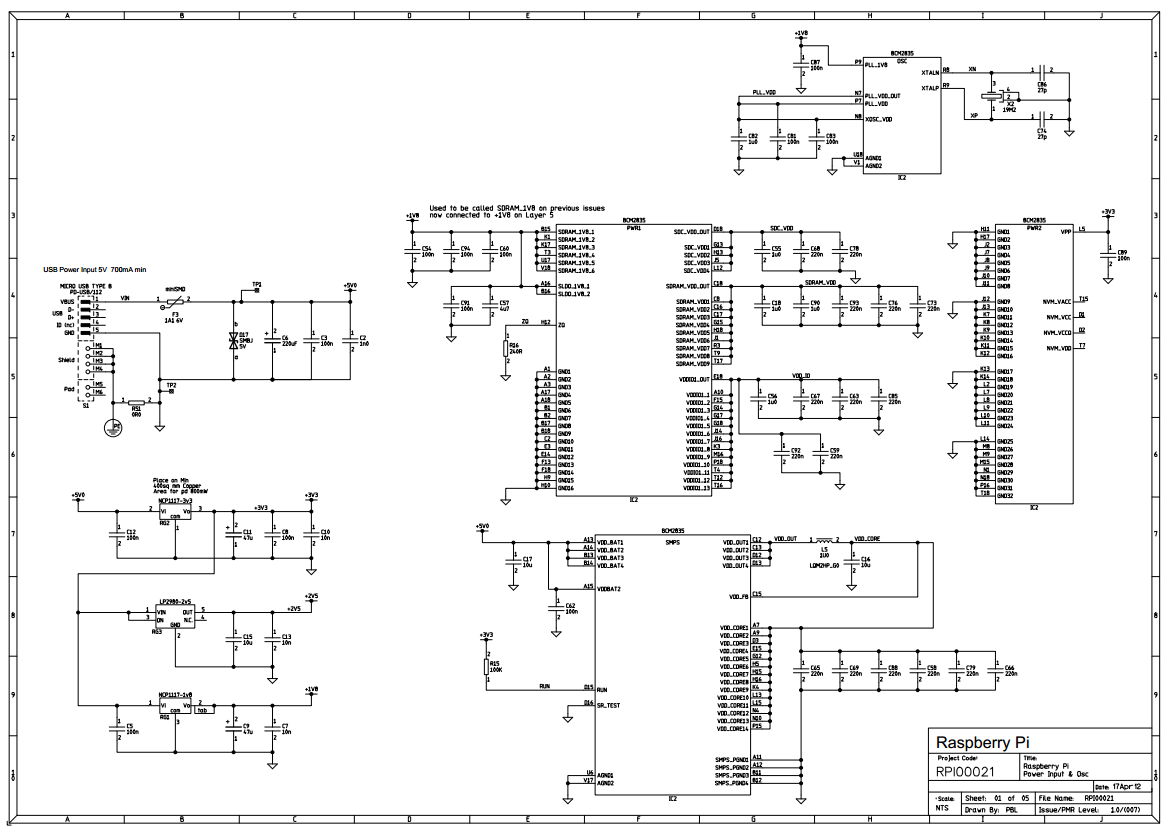
\includegraphics[width = \textwidth]{036}
    \caption{树莓派3B电路图}\par
\end{figure}
\subsubsection{飞控板}
飞控板控制的电机,是机器人最主要的动力来源,重要性不亚于单片机。经过考虑,我们决定采用APM2.8飞控板。
\begin{figure}[H]
\centering
    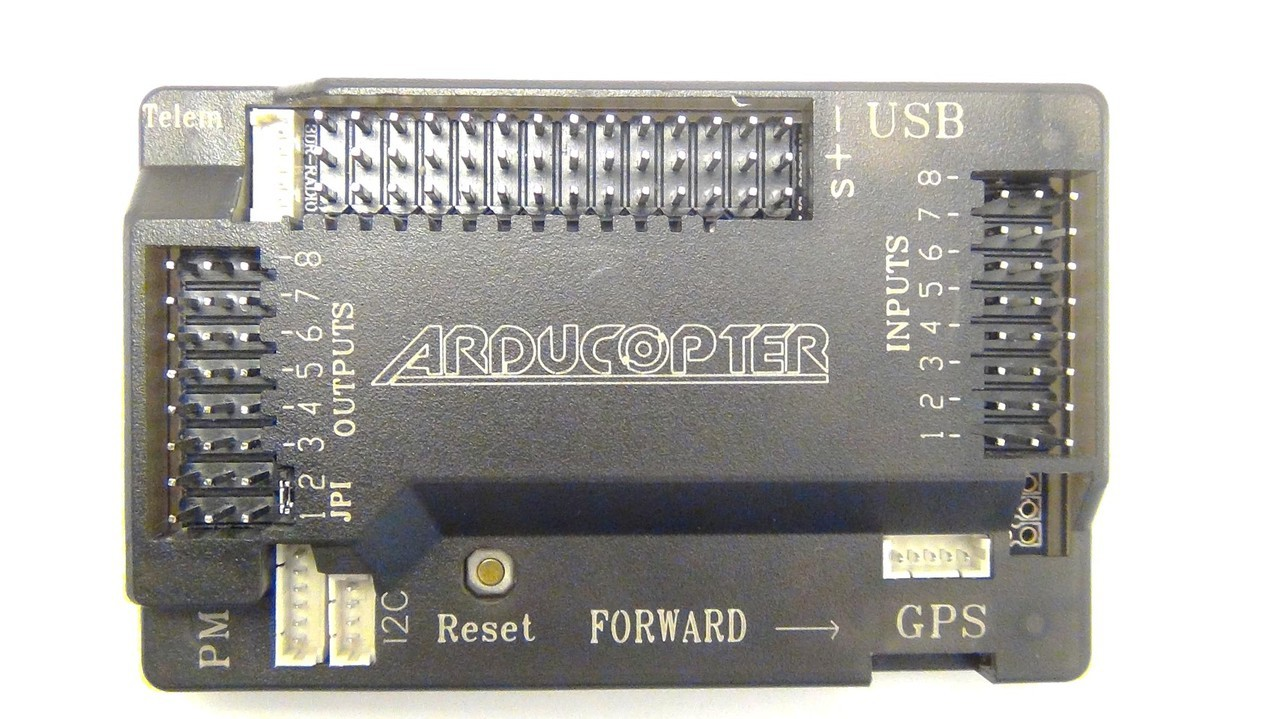
\includegraphics[width = \textwidth]{037}
    \caption{飞控板实物图}\par
\end{figure}
\begin{figure}[H]
\centering
    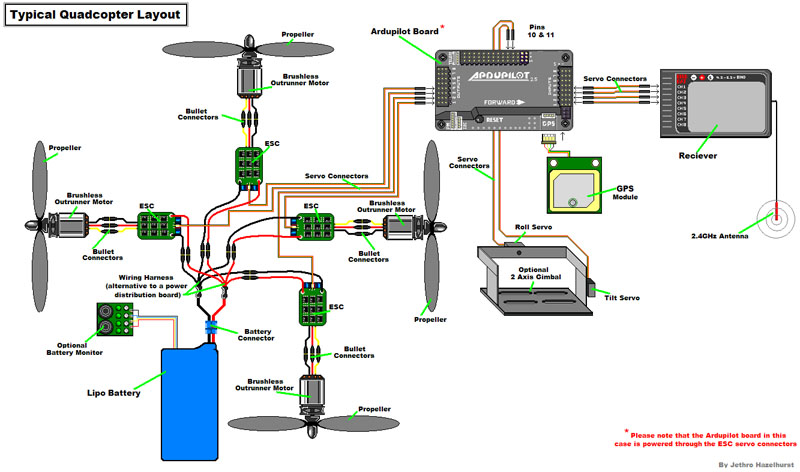
\includegraphics[width = \textwidth]{038}
    \caption{飞控板接口图}\par
\end{figure}
\begin{center}
\begin{itemize}
\item 1 x 3轴陀螺仪
\item 1 x加速计
\item 1 x磁力计
\item 1 x气压计
\item 4MB板上数据缓存芯片
\item  ATMEGA2560 和ATMEGA32U-2芯片
\item 尺寸:61 x 41 x 89mm
\item 重量:53.86g
\end{itemize}
\end{center}

\subsection{程序控制}
程序控制主要实现两种功能:室内定位和飞行控制。
\subsubsection{室内定位}
一般无人机的定位都是基于飞控板的GPS接口,然后通过接收卫星发出的GPS信号实现定位。然而,由于钢筋混凝土的遮挡,室内基本不能接受到GPS卫星信号。即便偶尔可以接收到,信号也没有室外那么稳定,可能会出现时断时续、精度下降的现象。而无人机定位需要比较好的实时性及准确性,需要避免这种情况的出现,所以我们必须通过其它的方法来实现室内定位。\par
实现方法:基于超声波测距的定位。\par
\begin{figure}[H]
\centering
    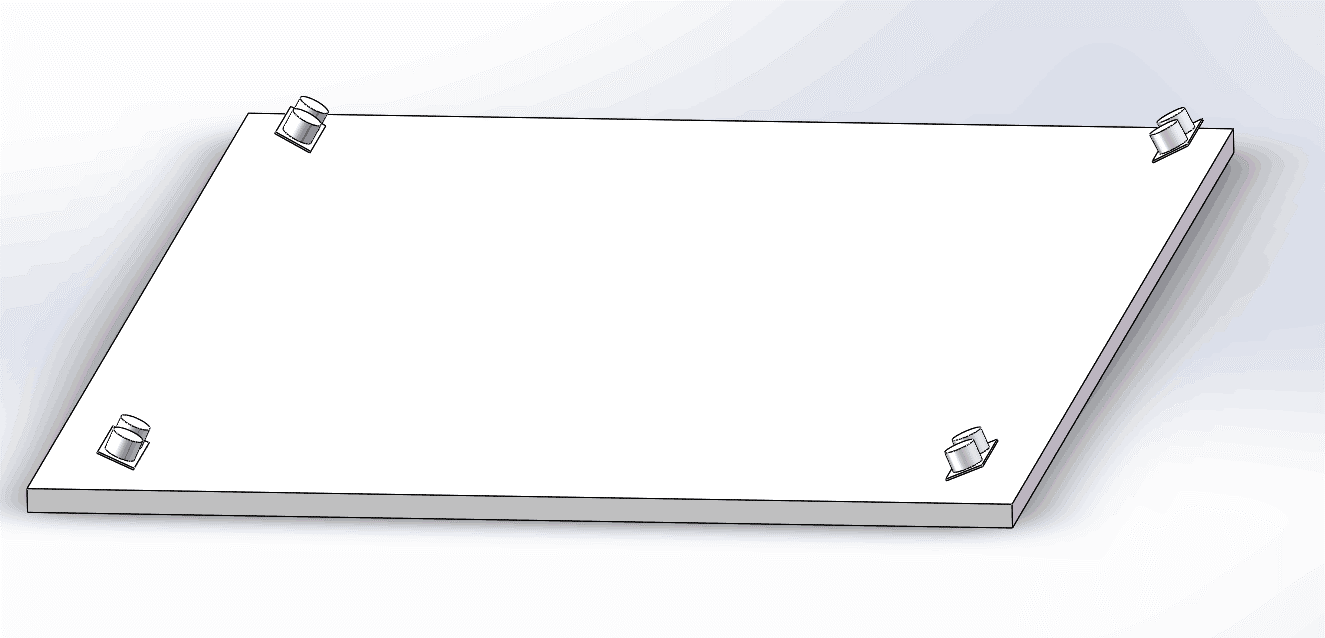
\includegraphics[width = \textwidth]{039}
    \caption{超声波接收器安置图}\par
\end{figure}
如图所示,在地面放置四个超声波接收器,四个接收器构成一个正方形,坐标记为A1(0,a), A2(0,0), A3(a,0), A4(a,a)。分别测量超声波发射器与四个接收器的距离,根据测量得到的距离用程序计算。程序如下:(C语言实现)
\begin{lstlisting}
\#include <stdio.h>
\#include <math.h>
\#include <stdlib.h>

typedef struct{
	double x;
	double y;
	double height;
}position,*posinf;//储存位置信息

const double a=1;//接收器构成正方形的边长,可修改

posinf calpos(double s1,double s2,double s3,double s4)/*si为发射器到接收器Ai的距离*/
\{
	int i;
	posinf b;
	double o23=0,o34=0,o14=0,o21=0;/*角度*/
	double x1=0,x2=0,y1=0,y2=0;/*坐标*/
	double h[4],s[4]={s1,s2,s3,s4};
	BOOL invalid=FALSE;
	b=(posinf)malloc(sizeof(position));
	if(b==NULL)exit(-1);
	b->x=0;
	b->y=0;
	b->height=0;
	o23=pow(s2,2)+pow(a,2)-pow(s3,2);
	o23/=2*s2*a;
	o23=acos(o23);
	o34=pow(s3,2)+pow(a,2)-pow(s4,2);
	o34/=2*s3*a;
	o34=acos(o34);
	o14=pow(s1,2)+pow(a,2)-pow(s4,2);
	o14/=2*s1*a;
	o14=acos(o14);
	o21=pow(s2,2)+pow(a,2)-pow(s1,2);
	o21/=2*s2*a;
	o21=acos(o21);
	x1=s2*cos(o23);
	x2=s1*cos(o14);
	y1=s3*cos(o34);
	y2=s2*cos(o21);
	if(s1<0)\{b->x=x1;b->y=y1;\}
	else if(s2<0)\{b->x=x2;b->y=y1;\}
	else if(s3<0)\{b->x=x2;b->y=y2;\}
	else if(s4<0)\{b->x=x1;b->y=y2;\}
	else\{
		b->x=(x1+x2)/2;
		b->y=(y1+y2)/2;
		\}
	h[1]=pow(s2,2)-pow(b->x,2)-pow(b->y,2);
	h[1]=sqrt(h1);
	h[0]=pow(s1,2)-pow(b->x,2)-pow(a-b->y,2);
	h[0]=sqrt(h0);
	h[3]=pow(s4,2)-pow(a-b->x,2)-pow(a-b->y,2);
	h[3]=sqrt(h3);
	h[2]=pow(s3,2)-pow(a-b->x,2)-pow(b->y,2);
	h[2]=sqrt(h2);
	for(i=0;i<4;i++)\{
		if(s[i]<0){invalid=TRUE;continue;\}
		else b->height+=h[i];
	\}
	if(invalid==TRUE)b->height/=3;
	else b->height/=4;
	return b;
\}

\end{lstlisting}

其实,只需要三个接收器就已经可以计算出位置,我们依旧选择额外增加一个接收器,原因有如下两个:\par
\begin{enumerate}
\item 对每个接收器,超声波测距会产生0.5\%的误差,在某些情况下会达到单个传感器2.5cm的误差。使用四个接收器可以计算出多个坐标取平均值,以减小误差,实现更精确的定位,从而实现更精确的控制。\par
\item 超声波测距的有效距离为5m,而这个距离有一些小,不能满足场地的需求。而使用四个接收器时,可以使机器人移动到其中一个接收器接收有效信号的范围之外,这样就增大了控制的范围(当其中一个接收不到信号时,定义该传感器的测量值为负,程序根据其余的三个距离计算出位置)。
\end{enumerate}
\subsubsection{飞行控制}
飞行控制是机器人最关键的部分,主要需要实现以下几个功能:降落、避障、跟随。\par
-降落\par
	机器降落时,要调整电机的转速,使电机的转速处在一个合适的区间,不能过高或过低。过高会使的机器下降极为缓慢,而过低会使得机器下落过快,在落地时可能会对机器造成损伤。\par
	实现机器平稳降落,只需要基于前面的定位,根据位置信息计算下落速度,程序自动调整电机转速,达到平稳降落的目的。\par
-避障\par
	避障基于光电传感器,机器四周的光电传感器实时测距,根据周围物体的距离自动调整路径。\par
-跟随\par
	跟随基于图像识别(使用OpenCV实现)。首先要查找轮廓(一般对应一系列点),然后存储轮廓(在OpenCV中一般使用序列来存储轮廓信息,其中每一个元素是一个点的位置)。要进行跟随时,进行轮廓的匹配。由于我们并不需要特别精确的匹配,所以采用最简单的方法:比较轮廓矩。\par
	轮廓矩定义如下:\par
\[mp,q = \sum\limits_{i = 1}^n {I(x,y){x^p}{y^q}} \]\par
	其中p对应x维度上的矩,q对应y维度,阶数表示对应部分的指数。即为对轮廓边界上所有像素进行求和。\par
	匹配后,进行跟踪。首先要寻找角点(独一无二的特殊点),然后跟踪角点,根据光流将目标物体的运动转换成速度矢量,经过计算之后,转换成机器人的运动,传输至单片机,然后控制机器人改变运动方向。\par

\section{经费预估}
\begin{center}
\begin{longtable}{|c|c|c|c|}
\hline
事由&	单价	&数量	&合计\\
\hline
4000mAh 锂聚合物电池	&337	&1	&337\\
\hline
E3F-DS30C4 红外线光电传感器	&16&	6(一个备用)	&96\\
\hline
TELESKY HC-SR04超声波传感器	&4	&6(一个备用)	&24\\
\hline
EZVIZ C3C无线网络摄像头	&249	&1	&249\\
\hline
APM2.8飞控板	&299	&1	&299\\
\hline
"WS9130KT机专用无刷电机1400kv、30A电调"	&85&	5	&425\\
\hline
3K 碳纤维管 22*20*1000mm	&70	&2	&140\\
\hline
3K 碳纤维管12*18*1000mm	&21	&6	&126\\
\hline
200 x 300mm 3K碳纤维板 1.5mm	&109	&3	&327\\
\hline
1.65米雨伞骨架	&100	&1	&100\\
\hline
树莓派3代B型	&215	&1	&215\\
\hline
自紧桨螺旋桨叶	&49&	2	&98\\
\hline
材料加工费		&&&	400\\
\hline
电子器件	&&&		500\\
\hline
安装座、轴承等零件	&&&		300\\
\hline
SG90 9G舵机	&7	&4	&28\\
\hline
荧光粉	&6	&1	&6\\
\hline
led裸板灯带	&3&	5	&15\\
\hline
塑料薄膜	&2	&2	&4\\
\hline
尼龙带	&8	&1	&8\\
\hline
			&&&3697\\
			\hline

\end{longtable}
\end{center}

\section{时间安排}
\centering
\begin{center}
\begin{longtable}{|c|c|}
\hline
7月1日——7月10日&积极参加机器人培训,队员深入学习各自领域知识,\\
&准备制作材料\\
\hline
7月11日——8月14日&开始动手制作机器人,完成机械与电路部分的制作,\\
&同时初步程序框架完成。完善机器人的功能要求。\\
\hline
8月15日——9月17日&对机器人调试,改善机器人性能,完整实现各功能\\
\hline
9月18日——9月24日&调试机器人的表演动作,提高稳定性,并进行实地彩排\\
\hline
\end{longtable}
\end{center}


\bibliography{report}
\bibliographystyle{plain}
\end{document}